% ==============================================================================
% Modelo para Monografia de Projeto de Graduação (PG)
% Prof. Vítor E. Silva Souza - Nemo / DI / UFES
%
% Baseado em abtex2-modelo-trabalho-academico.tex, v-1.9.2 laurocesar
% Copyright 2012-2014 by abnTeX2 group at http://abntex2.googlecode.com/ 
%
% This work may be distributed and/or modified under the conditions of the LaTeX 
% Project Public License, either version 1.3 of this license or (at your option) 
% any later version. The latest version of this license is in
% http://www.latex-project.org/lppl.txt.
%
% IMPORTANTE:
% Instruções encontram-se espalhadas pelo documento. Para facilitar sua leitura,
% tais instruções são precedidas por (*) -- utilize a função localizar do seu
% editor para passar por todas elas.
% ==============================================================================

% Usa o estilo abntex2, configurando detalhes de formatação e hifenização.
\documentclass[
	12pt,				% Tamanho da fonte.
	openright,			% Capítulos começam em página ímpar (insere página vazia caso preciso).
	oneside,			% Para impressão em verso e anverso. Oposto a oneside.
	a4paper,			% Tamanho do papel.
	english,			% Idioma adicional para hifenização.
	french,				% Idioma adicional para hifenização.
	spanish,			% Idioma adicional para hifenização.
	brazil				% O último idioma é o principal do documento.
	]{abntex2}



%%% Importação de pacotes. %%%

% Conserta o erro "No room for a new \count". 
% O comando \reserveinserts deve ser comentado ou não, dependendo da versão do LaTeX.
\usepackage{etex}
%\reserveinserts{28}

% Usa a fonte Latin Modern.
\usepackage{lmodern}

% Seleção de códigos de fonte.
\usepackage[T1]{fontenc}

% Codificação do documento em Unicode.
\usepackage[utf8]{inputenc}

% Usado pela ficha catalográfica.
\usepackage{lastpage}

% Indenta o primeiro parágrafo de cada seção.
\usepackage{indentfirst}

% Controle das cores.
\usepackage[usenames,dvipsnames]{xcolor}

% Inclusão de gráficos.
\usepackage{graphicx}

% Tabularx package: melhor controle de leiaute de tabelas.
\usepackage{tabularx}

% Inclusão de páginas em PDF diretamente no documento (para uso nos apêndices).
\usepackage{pdfpages}

% Para melhorias de justificação.
\usepackage{microtype}

% Citações padrão ABNT.
\usepackage[brazilian,hyperpageref]{backref}
\usepackage[alf]{abntex2cite}	
\renewcommand{\backrefpagesname}{Citado na(s) página(s):~}		% Usado sem a opção hyperpageref de backref.
\renewcommand{\backref}{}										% Texto padrão antes do número das páginas.
\renewcommand*{\backrefalt}[4]{									% Define os textos da citação.
	\ifcase #1
		Nenhuma citação no texto.
	\or
		Citado na página #2.
	\else
		Citado #1 vezes nas páginas #2.
	\fi}

% \rm is deprecated and should not be used in a LaTeX2e document
% http://tex.stackexchange.com/questions/151897/always-textrm-never-rm-a-counterexample
\renewcommand{\rm}{\textrm}

% Inclusão de símbolos não padrão.
\usepackage{amssymb}
\usepackage{eurosym}

% Para utilizar \eqref para referenciar equações.
\usepackage{amsmath}

% Permite mostrar figuras muito largas em modo paisagem com \begin{sidewaysfigure} ao invés de \begin{figure}.
\usepackage{rotating}

% Permite customizar listas enumeradas/com marcadores.
\usepackage{enumitem}

% Permite inserir hiperlinks com \url{}.
\usepackage{bigfoot}
\usepackage{hyperref}

% Permite usar o comando \hl{} para evidenciar texto com fundo amarelo. Útil para chamar atenção a itens a fazer.
\usepackage{soulutf8}

% Colorinlistoftodos package: to insert colored comments so authors can collaborate on the content.
\usepackage[colorinlistoftodos, textwidth=20mm, textsize=footnotesize]{todonotes}
\newcommand{\aluno}[1]{\todo[author=\textbf{Aluno},color=green!30,caption={},inline]{#1}}
\newcommand{\professor}[1]{\todo[author=\textbf{Professor},color=red!30,caption={},inline]{#1}}

% Permite inserir espaço em branco condicional (incluído no texto final só se necessário) em macros.
\usepackage{xspace}

% Permite incluir listagens de código com o comando \lstinputlisting{}.
\usepackage{listings}
\usepackage{caption}
\DeclareCaptionFont{white}{\color{white}}
\DeclareCaptionFormat{listing}{\colorbox{gray}{\parbox{\textwidth}{#1#2#3}}}
\captionsetup[lstlisting]{format=listing,labelfont=white,textfont=white}
\renewcommand{\lstlistingname}{Listagem}
\definecolor{mygray}{rgb}{0.5,0.5,0.5}
\lstset{
	basicstyle=\scriptsize,
	breaklines=true,
	numbers=left,
	numbersep=5pt,
	numberstyle=\tiny\color{mygray}, 
	rulecolor=\color{black},
	showstringspaces=false,
	tabsize=2,
    inputencoding=utf8,
    extendedchars=true,
    literate=%
    {é}{{\'{e}}}1
    {è}{{\`{e}}}1
    {ê}{{\^{e}}}1
    {ë}{{\¨{e}}}1
    {É}{{\'{E}}}1
    {Ê}{{\^{E}}}1
    {û}{{\^{u}}}1
    {ù}{{\`{u}}}1
    {â}{{\^{a}}}1
    {à}{{\`{a}}}1
    {á}{{\'{a}}}1
    {ã}{{\~{a}}}1
    {Á}{{\'{A}}}1
    {Â}{{\^{A}}}1
    {Ã}{{\~{A}}}1
    {ç}{{\c{c}}}1
    {Ç}{{\c{C}}}1
    {õ}{{\~{o}}}1
    {ó}{{\'{o}}}1
    {ô}{{\^{o}}}1
    {Õ}{{\~{O}}}1
    {Ó}{{\'{O}}}1
    {Ô}{{\^{O}}}1
    {î}{{\^{i}}}1
    {Î}{{\^{I}}}1
    {í}{{\'{i}}}1
    {Í}{{\~{Í}}}1
}



%%% Definição de variáveis. %%%

% (*) Substituir os textos abaixo com as informações apropriadas.
\titulo{Aplicação do método FrameWeb no desenvolvimento do
sistema SCAP utilizando os frameworks GWT e Grails}
\autor{Leonardo Nascimento dos Santos}
\local{Vitória, ES}
\data{2020}
\orientador{Prof. Dr. Vítor E. Silva Souza}
%\coorientador{Nome do Co-orientador}
\instituicao{
  Universidade Federal do Espírito Santo -- UFES
  \par
  Centro Tecnológico
  \par
  Departamento de Informática}
\tipotrabalho{Monografia (PG)}

% Preâmbulo (tipo do trabalho, objetivo, nome da instituição, área de concentração, etc.).
% (*) Verificar se está correto (ex.: substituir por Engenharia de Computação se for o caso).
\preambulo{Monografia apresentada ao Curso de Ciência da Computação do Departamento de Informática da Universidade Federal do Espírito Santo, como requisito parcial para obtenção do Grau de Bacharel em Ciência da Computação.}

% Macros específicas do trabalho.
% (*) Inclua aqui termos que são utilizados muitas vezes e que demandam formatação especial.
% Os exemplos abaixo incluem i* (substituindo o asterisco por uma estrela) e Java com TM em superscript.
% Use sempre \xspace para que o LaTeX inclua espaço em branco após a macro somente quando necessário.
\newcommand{\istar}{\textit{i}$^\star$\xspace}
\newcommand{\java}{Java\texttrademark\xspace}
\newcommand{\latex}{\LaTeX\xspace}




%%% Configurações finais de aparência. %%%

% Altera o aspecto da cor azul.
\definecolor{blue}{RGB}{41,5,195}

% Informações do PDF.
\makeatletter
\hypersetup{
	pdftitle={\@title}, 
	pdfauthor={\@author},
	pdfsubject={\imprimirpreambulo},
	pdfcreator={LaTeX with abnTeX2},
	pdfkeywords={abnt}{latex}{abntex}{abntex2}{trabalho acadêmico}, 
	colorlinks=true,				% Colore os links (ao invés de usar caixas).
	linkcolor=blue,					% Cor dos links.
	citecolor=blue,					% Cor dos links na bibliografia.
	filecolor=magenta,				% Cor dos links de arquivo.
	urlcolor=blue,					% Cor das URLs.
	bookmarksdepth=4
}
\makeatother

% Espaçamentos entre linhas e parágrafos.
\setlength{\parindent}{1.3cm}
\setlength{\parskip}{0.2cm}



%%% Páginas iniciais do documento: capa, folha de rosto, ficha, resumo, tabelas, etc. %%%

% Compila o índice.
\makeindex

% Inicia o documento.
\begin{document}

% Retira espaço extra obsoleto entre as frases.
\frenchspacing

% Capa do trabalho.
\imprimircapa

% Folha de rosto (o * indica que haverá a ficha bibliográfica).
\imprimirfolhaderosto*


% Ficha catalográfica.
% (*) Escolher entre as versões de ficha catalográfica abaixo (comente aquela que não quiser usar).

% Versão 1: caso a biblioteca da sua universidade lhe forneça um PDF (adequar o nome do arquivo).
% \begin{fichacatalografica}
%     \includepdf{include-fichacatalografica.pdf}
% \end{fichacatalografica}

% Versão 2: caso você tenha que inserir sua própria ficha catalográfica.
% (*) Neste caso, preencher palavras-chave e adicione co-orientador (se houver).
\begin{fichacatalografica}
	\vspace*{\fill}
	\hrule
	\begin{center}
	\begin{minipage}[c]{12.5cm}
	
	\imprimirautor
	
	\hspace{0.5cm} \imprimirtitulo  / \imprimirautor. --
	\imprimirlocal, \imprimirdata-
	
	\hspace{0.5cm} \pageref{LastPage} p. : il. (algumas color.) ; 30 cm.\\
	
	\hspace{0.5cm} \imprimirorientadorRotulo~\imprimirorientador\\
	
	\hspace{0.5cm}
	\parbox[t]{\textwidth}{\imprimirtipotrabalho~--~\imprimirinstituicao,
	\imprimirdata.}\\
	
	\hspace{0.5cm}
		1. Palavra-chave1.
		2. Palavra-chave2.
		I. Souza, Vítor Estêvão Silva.
		II. Universidade Federal do Espírito Santo.
		IV. \imprimirtitulo \\ 			
	
	\hspace{8.75cm} CDU 02:141:005.7\\
	
	\end{minipage}
	\end{center}
	\hrule
\end{fichacatalografica}


% Folha de aprovação.
% (*) Escolher entre as versões de ficha catalográfica abaixo (comente aquela que não quiser usar).

% Versão 1: cópia digitalizada da folha de aprovação assinada pela banca.
% \includepdf{include-folhadeaprovacao.pdf}

% Versão 2: folha de aprovação em branco.
% (*) Ajustar a data e os nomes dos participantes da banca.
\begin{folhadeaprovacao}
  \begin{center}
    {\ABNTEXchapterfont\large\imprimirautor}
    \vspace*{\fill}\vspace*{\fill}
    \begin{center}
      \ABNTEXchapterfont\bfseries\Large\imprimirtitulo
    \end{center}
    \vspace*{\fill}
    \hspace{.45\textwidth}
    \begin{minipage}{.5\textwidth}
        \imprimirpreambulo
    \end{minipage}%
    \vspace*{\fill}
   \end{center}
   Trabalho aprovado. \imprimirlocal, ? de ? de 2019:
   \assinatura{\textbf{\imprimirorientador} \\ Orientador} 
   \assinatura{\textbf{Professor} \\ Convidado 1}
   \assinatura{\textbf{Professor} \\ Convidado 2}
   %\assinatura{\textbf{Professor} \\ Convidado 3}
   %\assinatura{\textbf{Professor} \\ Convidado 4}
   \begin{center}
    \vspace*{0.5cm}
    {\large\imprimirlocal}
    \par
    {\large\imprimirdata}
    \vspace*{1cm}
  \end{center}  
\end{folhadeaprovacao}


% Dedicatória.
% (*) Escrever dedicatória ou remover/comentar seção.
\begin{dedicatoria}
   \vspace*{\fill}
   \centering
   \noindent
   \textit{A Deus e os meus pais que são tudo em minha vida.} \vspace*{\fill}
\end{dedicatoria}


% Agradecimentos.
% (*) Escrever agradecimentos ou remover/comentar seção.
\begin{agradecimentos}
Agradeço a Deus por ser o primeiro em minha vida. Sem Deus eu não teria forças para superar todas as barreiras enfrentadas durante esses anos.

Aos meus pais, Neilson Nascimento dos Santos e Angela Maria Nascimento dos Santos, que me deram todo o amor incondicional que um filho poderia ter. Meus pais nunca deixaram que nada me faltasse e me deram total apoio nas decisões que tomei. Por esse motivo, espero conseguir retribuir da mesma maneira para que nada falte para eles também.

À minha namorada, Isabela Valim Sarmento, por todo o amor, carinho, por compartilhar comigo inúmeros momentos inesquecíveis, por ser minha amiga e estar do meu lado em tudo.
 
Também agradeço aos meus “irmãos”, Vinícius Berger e Gustavo Costa Duarte, pois não é preciso ter irmãos de sangue para se construir uma amizade verdadeira. Eles foram peças fundamentais para que eu conseguisse chegar nesse momento tão importante.

Agradeço aos meus amigos, Igor de Moura Ventorim, Gustavo Epichin Monjardim e Eduardo Gorayeb Dalapicola, por sempre me ajudarem durante a minha graduação. Obrigado a todos os meus colegas e todas as pessoas boas que conheci na universidade.

Obrigado a todos os professores que contribuíram para a minha formação, em especial Rosane, Eduardo, Ricardo, Davidson e principalmente o meu orientador Vítor, que me transmitiu um conhecimento inestimável.
\end{agradecimentos}


% Epígrafe.
% (*) Escrever epígrafe ou remover/comentar seção.
\begin{epigrafe}
    \vspace*{\fill}
	\begin{flushright}
		\textit{``Mas buscai primeiro o Reino de Deus, \\
		e a sua Justiça, e as demais coisas vos serão acrescentadas.'' \\
		(Jesus Cristo)}
	\end{flushright}
\end{epigrafe}


% Resumo em português.
% (*) Escrever resumo e palavras-chave.
\setlength{\absparsep}{18pt}
\begin{resumo}
Lorem ipsum dolor sit amet, consectetur adipiscing elit. Duis malesuada laoreet leo at interdum. Nullam neque eros, dignissim sed ipsum sed, sagittis laoreet nisi. Duis a pulvinar nisl. Aenean varius nisl eu magna facilisis porttitor. Cum sociis natoque penatibus et magnis dis parturient montes, nascetur ridiculus mus. Ut mattis tortor nisi, facilisis molestie arcu hendrerit sed. Donec placerat velit at odio dignissim luctus. Suspendisse potenti. Integer tristique mattis arcu, ut venenatis nulla tempor non. Donec at tincidunt nulla. Cras ac dignissim neque. Morbi in odio nulla. Donec posuere sem finibus, auctor nisl eu, posuere nisl. Duis sit amet neque id massa vehicula commodo dapibus eu elit. Sed nec leo eu sem viverra aliquet. Nam at nunc nec massa rutrum aliquam sed ac ante.

Vivamus nec quam iaculis, tempus ipsum eu, cursus ante. Phasellus cursus euismod auctor. Fusce luctus mauris id tortor cursus, volutpat cursus lacus ornare. Proin tristique metus sed est semper, id finibus neque efficitur. Cras venenatis augue ac venenatis mollis. Maecenas nec tellus quis libero consequat suscipit. Aliquam enim leo, pretium non elementum sit amet, vestibulum ut diam. Maecenas vitae diam ligula.

Fusce ac pretium leo, in convallis augue. Mauris pulvinar elit rhoncus velit auctor finibus. Praesent et commodo est, eu luctus arcu. Vivamus ut porta tortor, eget facilisis ex. Nunc aliquet tristique mauris id sollicitudin. Donec quis commodo metus, sit amet accumsan nibh. Cum sociis natoque penatibus et magnis dis parturient montes, nascetur ridiculus mus.

Duis elementum dictum tristique. Integer mattis libero sit amet pretium euismod. Curabitur auctor eu augue ut ornare. Integer bibendum eros ullamcorper rhoncus convallis. Pellentesque non pretium ligula, sit amet bibendum eros. Nam venenatis ex felis, quis blandit nunc auctor sit amet. Maecenas ut eros pharetra, lobortis neque id, fermentum arcu. Cras neque dui, rhoncus feugiat leo id, semper facilisis lorem. Fusce non ex turpis. Nullam venenatis sed ligula ac lacinia.

\textbf{Palavras-chaves}: lorem. ipsum. dolor. sit. amet.
\end{resumo}

% Insere lista de ilustrações.
\pdfbookmark[0]{\listfigurename}{lof}
\listoffigures*
\cleardoublepage

% Insere lista de tabelas.
\pdfbookmark[0]{\listtablename}{lot}
\listoftables*
\cleardoublepage

% Lista de abreviaturas e siglas.
% (*) Preencher com as siglas usadas ao longo do texto e seus significados.
\begin{siglas}
	\item [UML] Linguagem de Modelagem Unificada, do inglês \textit{Unified Modeling Language}
	\item [SCAP] Sistema de Controle de Afastamento de Professores
	\item [WIS] \textit{Web-based Information Systems}
	\item [WWW] \textit{World Wide Web}
	\item [ABNT] Associação Brasileira de Normas Técnicas
\end{siglas}

% Insere o sumário.
\pdfbookmark[0]{\contentsname}{toc}
\tableofcontents*
\cleardoublepage



%%% Início da parte de conteúdo do documento. %%%

% Marca o início dos elementos textuais.
\textual

% Inclusão dos capítulos.
% (*) Para facilitar a organização, os capítulos foram divididos em arquivo separados e colocados dentro da.
% pasta capitulos/. Caso o aluno prefira trabalhar com um só arquivo, basta substituir os comandos \include 
% pelos conteúdos dos arquivos que estão sendo incluídos, excluindo a pasta capitulos/ em seguida.
% ==============================================================================
% TCC - Nome do Aluno
% Capítulo 1 - Introdução
% ==============================================================================
\chapter{Introdução}
\label{sec-intro}

Antigamente, os servidores não comportavam páginas \textit{Web} que continham um conteúdo muito denso. Funcionando apenas com páginas estáticas, realizar manutenções e controle das funcionalidades era uma tarefa muito difícil. Com o desenvolvimento de novas tecnologias a partir da criação da \textit{World Wide Web} (WWW) e através do surgimento de novas linguagens de programação para a \textit{Web}, os servidores tiveram que ser adaptados para se tornarem mais robustos. Com a infraestrutura de software modificada, os servidores começaram a aceitar páginas dinâmicas que passaram a ser carregadas de conteúdos que antes não eram suportados e isso também possibilitou que essas páginas possuíssem efeitos diversos, tais como animações de conteúdo.

Ainda nessa constante evolução, sistemas projetados para serem utilizados a partir de um navegador ou de aplicativos, puderam ser criados de uma maneira em que os servidores processassem e retornassem as informações para os visitantes através da Internet, surgindo assim o conceito de \textit{WebApp}, ou aplicação \textit{Web}. Lojas virtuais e sistemas de fornecimento entre empresas são exemplos de \textit{websites} que puderam ser desenvolvidos por meio de \textit{WebApps}. Desta maneira, o foco deste trabalho serão os Sistemas de Informação Baseados na \textit{Web (Web-based Information Systems – WISs)}, que são enquadrados em uma categoria específica de \textit{WebApps}. Esses sistemas são caracterizados como sistemas de informação tradicionais, mas estão disponíveis na Internet.

Quando falamos sobre o desenvolvimento de \textit{WebApps} atuais, em particular os WISs, temos que entender que utilizar a Engenharia de Software é uma tarefa fundamental. Os aspectos relacionados ao estabelecimento de técnicas, processos, métodos, ferramentas e ambientes de suporte ao desenvolvimento de software são tratados de forma clara pela Engenharia de Software~\cite{falbo:es14}. Trazendo alguns benefícios como, por exemplo, a compatibilidade entre plataformas e a facilidade de gerenciamento, as \textit{WebApps} por meio dos servidores, se tornaram indispensáveis para manterem os serviços e as aplicações disponíveis em qualquer parte do mundo através da Internet.

No meio de tantas criações e adaptações tecnológicas, surge o uso de \textit{frameworks} para \textit{WebApps}. Se tornando uma das ferramentas mais importantes para o desenvolvimento de \textit{WebApps}, os \textit{frameworks} passaram a auxiliar no encapsulamento das funcionalidades de alto nível com maior eficiência e agilidade, fazendo com que a maior parte do tempo e do trabalho fossem economizados. Visando propor uma abordagem diferenciada para a construção de sistemas para \textit{Web}, surge então o método FrameWeb (\textit{Framework-based Design Method for Web Engineering})~\cite{souza:masterthesis07}. Com o intuito de utilizar diversos \textit{frameworks}, o método FrameWeb busca agilizar o desenvolvimento de \textit{WebApps}, minimizando as tarefas realizadas nas fases que a Engenharia de Software determina.

Baseado na linguagem de modelagem UML (Unifield Modeling Language)~\cite{booch-et-al:u06}, o método FrameWeb propõe quatro diagramas para a fase de projeto de software que incorporam os conceitos trazidos pelos \textit{frameworks} utilizados no desenvolvimento Web, de modo a facilitar a comunicação entre desenvolvedores, agilizar o desenvolvimento por meio de geração de código, dentre outras vantagens. Originalmente, o método se propunha a dar suporte a três categorias de \textit{frameworks}: controladores frontais, injeção de dependências e mapeamento objeto/relacional.

Existem, no entanto, inúmeros \textit{frameworks} existentes dentro de cada categoria. Sendo assim, se faz necessário experimentar o método com \textit{frameworks} diversos, avaliando sua adequação. Neste contexto, \citeonline{duarte-pg14} desenvolveu uma \textit{WebApp} --- um Sistema de Controle de Afastamento de Professores (SCAP) --- em seu trabalho de conclusão de curso. Esse sistema foi criado para apoiar um departamento de universidade a realizar um controle das solicitações de afastamento de seus professores efetivos. Utilizando os requisitos que foram levantados por \citeonline{duarte-pg14} e posteriormente analisados por \citeonline{prado-pg15}, este trabalho tem com tarefa fundamental a implementação do SCAP utilizando dois outros \textit{frameworks Web}, para que seja possível realizar a verificação da eficiência do método FrameWeb.

Os \textit{frameworks} experimentados neste trabalho serão o GWT e o Grails. O \textit{framework} GWT foi desenvolvido utilizando a linguagem de programação Java como base e em sua construção, foi adicionado um kit de ferramentas de desenvolvimento que facilita a otimização e criação de \textit{WebApps} que utilizam Ajax. O \textit{framework} Grails utiliza as linguagens de programação Java e Groovy, tendo como característica a minimização da complexidade da criação de \textit{WebApps} e podendo ser integrado com qualquer biblioteca Java através de plugins.

%\hrulefill

%Além do template pronto para uso, este documento inclui exemplos de uso de \latex que podem ser úteis para aqueles que possuem pouca experiência com a ferramenta. Quando for começar a escrever seu PG, apague todo o conteúdo abaixo da palavra ``Texto''.



%%% Início de seção. %%%
\section{Seções e subseções}
\label{sec-intro-secoes}

O documento é organizado em capítulos (\texttt{\textbackslash chapter\{\}}), seções (\texttt{\textbackslash section\{\}}), subseções (\texttt{\textbackslash subsection\{\}}), sub-subseções (\texttt{\textbackslash subsubsection\{\}}) e assim por diante. Atenção, porém, a não criar estruturas muito profundas (sub-sub-sub-...) pois o documento não fica bem estruturado.


%%% Início de seção. %%%
\subsection{Referências a seções}
\label{sec-intro-secoes-refs}

Cada parte do documento (capítulo, seção, etc.) deve possuir um rótulo logo abaixo de sua definição. Por exemplo, este capítulo é definido com \texttt{\textbackslash chapter\{Introdução\}} seguido por \texttt{\textbackslash label\{sec-intro\}}. Assim, podemos fazer referências cruzadas usando o comando \texttt{\textbackslash ref\{rótulo\}}: ``O Capítulo~\ref{sec-intro} começa com a Seção~\ref{sec-intro-secoes}, que é ainda subdividida nas subseções~\ref{sec-intro-secoes-refs} e~\ref{sec-intro-secoes-sobrerefs}.

Para melhor organização das partes do documento, sugere-se primeiro utilizar o prefixo \texttt{sec-} (para diferenciar de referências à figuras, tabelas, etc. quando usarmos o comando \texttt{\textbackslash ref\{\}}) e também representar a hierarquia das seções nos rótulos. Por exemplo, o Capítulo~\ref{sec-intro} tem rótulo \texttt{sec-intro}, sua Seção~\ref{sec-intro-secoes} tem rótulo \texttt{sec-intro-secoes} e a Subseção~\ref{sec-intro-secoes-refs} tem rótulo \texttt{sec-intro-secoes-refs}.



%%% Início de seção. %%%
\subsection{Sobre referências cruzadas}
\label{sec-intro-secoes-sobrerefs}

Nas próximas seções, veremos que é possível fazer referência cruzada não só a seções mas também a listagens de código, figuras, tabelas, etc. Em todos estes casos, quando nos referimos à Seção X, Listagem Y ou Figura Z, consideramos que estes são os nomes próprios destes elementos e, portanto, usa-se a primeira letra maiúscula. Isso pode ser visto na Subseção~\ref{sec-intro-secoes-refs}, acima. A exceção é quando nos referimos a vários elementos ao mesmo tempo, por exemplo: ``as subseções~\ref{sec-intro-secoes-refs} e~\ref{sec-intro-secoes-sobrerefs}''.

Por fim, ao usar o comando \texttt{\textbackslash ref\{\}}, sugere-se separá-lo da palavra que vem antes dele com um \textasciitilde\ ao invés de espaço. Por exemplo: \texttt{o capítulo\textasciitilde \textbackslash ref\{sec-intro\}}. Isso faz com que o \latex não quebre linha entre a palavra \texttt{capítulo} e o número do capítulo.




%%% Início de seção. %%%
\section{Citações bibliográficas}
\label{sec-intro-citacoes}

Este documento utiliza a ferramenta de gerenciamento de referências bibliográficas do \latex, chamada \emph{BibTeX}. O arquivo \texttt{bibliografia.bib}, referenciado no arquivo \latex principal deste documento, contém algumas referências bibliográficas de exemplo. Assim como capítulos, seções, etc., tais referências também possuem rótulos, especificados como primeiro parâmetro de cada entrada (ex.: \texttt{@incollection\{souza-et-al:iism08, ...\}}.

Sugere-se um padrão para rótulos de referências bibliográficas para que fique claro também no código \latex qual referência está sendo citada. Por exemplo, ao citar a referência \texttt{souza-et-al:sesas13}, sabemos que é um artigo escrito por \emph{Souza} e outros, publicado no \emph{SESAS} em \emph{2013} (geralmente a pessoa que citou sabe que publicação é SESAS e quem é Souza).

Para citar uma referência bibliográfica contida no arquivo \emph{BibTeX}, basta usar seu rótulo como parâmetro de um de dois comandos possíveis de citação:

\begin{itemize}
	\item O comando \texttt{\textbackslash cite\{\}} efetua uma citação tradicional, colocando o nome do(s) autor(es) e o ano entre parênteses. Por exemplo, \texttt{\textbackslash cite\{souza-et-al:iism08\}} é transformado em \cite{souza-et-al:iism08};
	
	\item O comando \texttt{\textbackslash citeonline\{\}} efetua uma citação integrada ao texto, colocando o nome do(s) autor(es) direto no texto e somente o ano entre parênteses. Por exemplo, ``de acordo com \texttt{\textbackslash citeonline\{souza-et-al:iism08\}}'' é transformado em: de acordo com \citeonline{souza-et-al:iism08};
\end{itemize}

Também é possível citar vários trabalhos de uma só vez, separando os rótulos das referências bibliográficas com uma vírgula dentro do comando apropriado. Por exemplo, \texttt{\textbackslash cite\{souza-et-al:sesas13,souza-et-al:csrd13\}} \cite{souza-et-al:sesas13,souza-et-al:csrd13}.

Os trabalhos citados são automaticamente incluídos na seção de referências bibliográficas, ao final do documento. Tudo é formatado automaticamente segundo padrões da ABNT.



%%% Início de seção. %%%
\section{Listagens de código}
\label{sec-intro-listagens}

O pacote \texttt{listings}, incluído neste template, permite a inclusão de listagens de código. Análogo ao já feito anteriormente, listagens possuem rótulos para que possam ser referenciadas e sugerimos uma regra de nomenclatura para tais rótulos: usar como prefixo o rótulo do capítulo, substituindo \texttt{sec-} por \texttt{lst-}.

A Listagem~\ref{lst-intro-exemplo}, por exemplo, possui o rótulo \texttt{lst-intro-exemplo} e representa o código que foi usado no próprio documento para exibir as listagens desta seção. Como podemos ver, a sugestão é que os arquivos de código sejam colocados dentro da pasta \texttt{codigos/} e tenham nome idêntico ao rótulo, colocando a extensão adequada ao tipo de código.

\lstinputlisting[label=lst-intro-exemplo, caption=Exemplo de código \latex para inclusão de listagens de código., float=htpb]{codigos/lst-intro-exemplo.tex}

A Listagem~\ref{lst-intro-outroexemplo} mostra um exemplo de listagem com especificação da linguagem utilizada no código. O pacote \texttt{listings} reconhece algumas linguagens\footnote{Veja a lista de linguagens suportadas em \url{http://en.wikibooks.org/wiki/LaTeX/Source\_Code\_Listings\#Supported_languages}.} e faz ``coloração'' de código (na verdade, usa \textbf{negrito} e não cores) de acordo com a linguagem. O parâmetro \texttt{float=htpb} incluído em ambos os exemplos impede que a listagem seja quebrada em diferentes páginas.

\lstinputlisting[label=lst-intro-outroexemplo, caption=Exemplo de código \java especificando linguagem utilizada., language=Java, float=htpb]{codigos/lst-intro-outroexemplo.java}



%%% Início de seção. %%%
\section{Figuras}
\label{sec-intro-figuras}

Figuras podem ser inseridas no documento usando o \emph{ambiente} \texttt{figure} (ou seja, \texttt{\textbackslash begin\{figure\}} e \texttt{\textbackslash end\{figure\}}) e o comando \texttt{\textbackslash includegraphics\{\}}. Existem alguns outros elementos e propriedades úteis de serem configuradas, resultando no código exibido na Listagem~\ref{lst-intro-figuras}.

\lstinputlisting[label=lst-intro-figuras, caption=Código \latex utilizado para inclusão das figuras na Seção~\ref{sec-intro-figuras}., float=htpb]{codigos/lst-intro-figuras.tex}

O comando \texttt{\textbackslash centering} centraliza a figura na página. A opção \texttt{width} do comando \texttt{\textbackslash includegraphics\{\}} determina o tamanho da figura e usa-se \texttt{\textbackslash textwidth} (opcionalmente multiplicado por um número) para se referir à largura da página.

O parâmetro do comando \texttt{\textbackslash includegraphics\{\}} indica onde a imagem pode ser encontrada. Foi criado o diretório \texttt{figuras/} para conter as figuras do documento, dando uma melhor organização aos arquivos. Ao abrir esta pasta, repare que as figuras possuem duas versões---uma em \texttt{.eps} e outra em \texttt{.pdf}---e que o comando \texttt{\textbackslash includegraphics\{\}} não especifica a extensão. Isso se dá porque o \latex possui um compilador para formato PostScript (\texttt{latex}) que espera as imagens em \texttt{.eps} e um compilador para PDF (\texttt{pdflatex}) que espera as imagens em \texttt{.pdf}. Dependendo do seu ambiente \latex, é possível apenas colocar as figuras em formatos mais comuns, como JPG ou PNG e ele incluir no PDF sem problemas. Vale a pena testar.

Por fim, o comando \texttt{\textbackslash caption\{\}} especifica a descrição da figura e \texttt{\textbackslash label\{\}}, como de costume, estabelece um rótulo para permitir referência cruzada de figuras. Note ainda que é utilizada a mesma estratégia de nomenclatura de rótulos usada nas listagens, porém utilizando o prefixo \texttt{fig-}.

As figuras~\ref{fig-intro-nemologo} e~\ref{fig-intro-exemplosideways} mostram o resultado do código da Listagem~\ref{lst-intro-figuras}. A Figura~\ref{fig-intro-exemplosideways}, em particular, utiliza o pacote \texttt{rotating} para mostrar figuras largas em modo paisagem. Basta usar o ambiente \texttt{sidewaysfigure} ao invés de \texttt{figure}.

\begin{figure}
	\centering
	
\includegraphics[width=.25\textwidth]{figuras/fig-intro-nemologo} 
	\caption{Exemplo de figura: logo do Nemo.}
	\label{fig-intro-nemologo}
\end{figure}

\begin{sidewaysfigure}
	\centering
	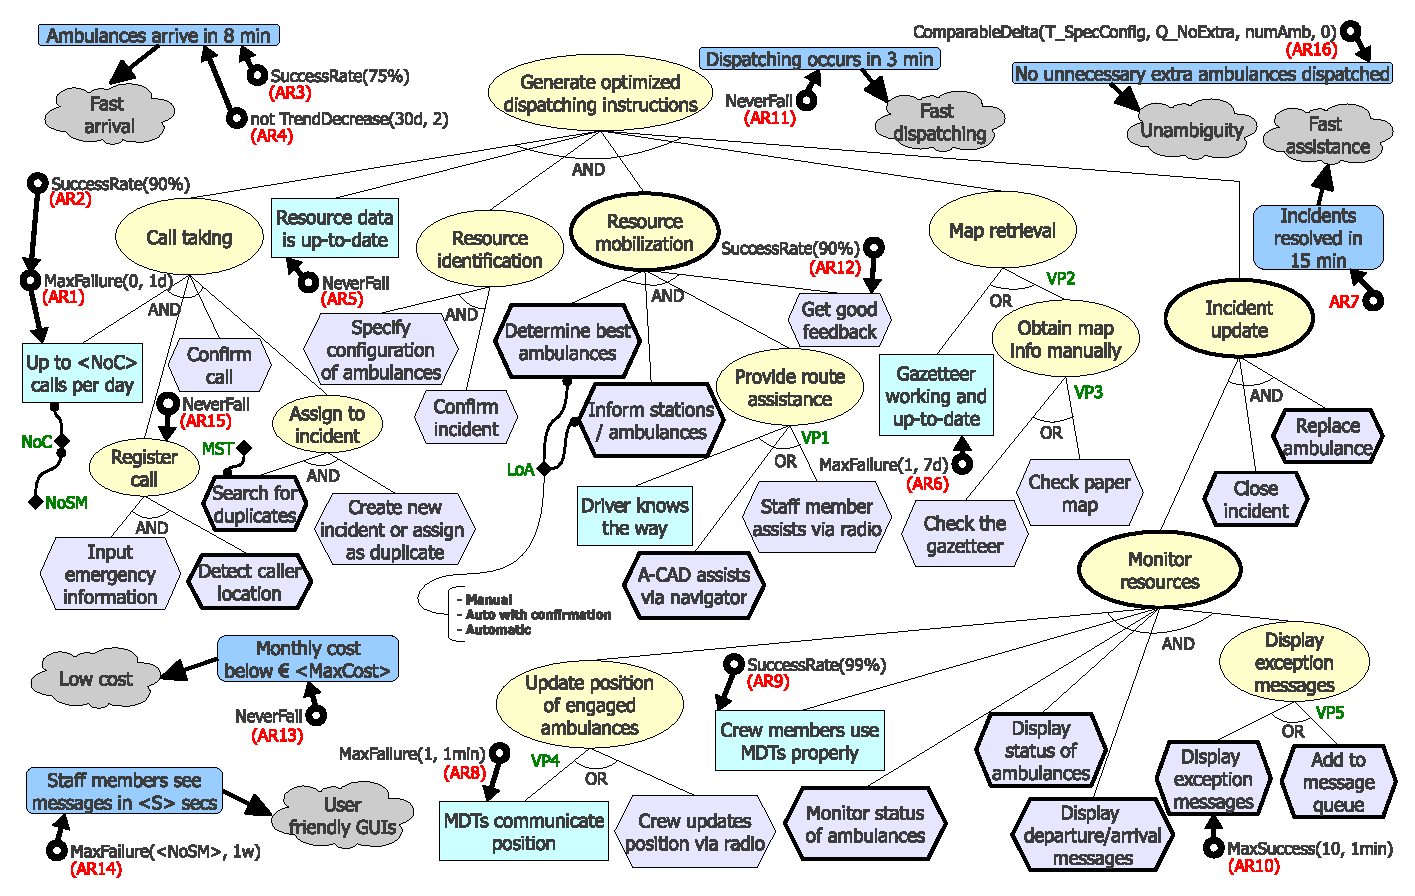
\includegraphics[width=\textwidth]{figuras/fig-intro-exemplosideways} 
	\caption{Exemplo de figura em modo paisagem: um modelo de objetivos~\cite{souza-mylopoulos:spe13}.}
	\label{fig-intro-exemplosideways}
\end{sidewaysfigure}



%%% Início de seção. %%%
\section{Tabelas}
\label{sec-intro-tabelas}

Tabelas são um ponto fraco do \latex. Elas são complicadas de fazer e, dependendo da complexidade da tabela (muitas células mescladas, por exemplo), vale a pena construi-las em outro programa (por exemplo, em seu editor de texto favorito) e inclui-las no documento como figuras. Mostramos, no entanto, alguns exemplos de tabela a seguir. O código utilizado para criar as tabelas encontra-se nas listagens~\ref{lst-intro-tabelas01}, \ref{lst-intro-tabelas02} e~\ref{lst-intro-tabelas03}.

\lstinputlisting[label=lst-intro-tabelas01, caption=Código \latex utilizado para inclusão das tabelas~\ref{tbl-intro-exemplo01} e~\ref{tbl-intro-exemplo02}., float=htpb]{codigos/lst-intro-tabelas01.tex}

\lstinputlisting[label=lst-intro-tabelas02, caption=Código \latex utilizado para inclusão da Tabela~\ref{tbl-intro-exemplo03}., float=htpb]{codigos/lst-intro-tabelas02.tex}

\lstinputlisting[label=lst-intro-tabelas03, caption=Código \latex utilizado para inclusão da Tabela~\ref{tbl-intro-exemplo04}., float=htpb]{codigos/lst-intro-tabelas03.tex}

Em particular, a Tabela~\ref{tbl-intro-exemplo04} utiliza um pacote chamado \texttt{tabularx}, que permite maior controle do layout das tabelas. Ao definir o ambiente \texttt{\textbackslash begin\{tabularx\}}, são definidos os tamanhos de cada coluna proporcional à largura ocupada pela tabela. Veja na Listagem~\ref{lst-intro-tabelas03} que as primeiras duas colunas não definem o atributo \texttt{\textbackslash hsize}, o que faz com que elas fiquem com o tamanho padrão de coluna, que é a largura da tabela dividida pelo número de colunas. Já a terceira coluna define \texttt{\textbackslash hsize=1.2\textbackslash hsize}, ou seja, esta coluna deve ser 20\% maior do que o tamanho padrão. Para isso, é preciso retirar de outras colunas, portanto a quarta e quinta colunas são definidas como 10\% menores (ou seja, \texttt{\textbackslash hsize=0.9\textbackslash hsize}).

% Exemplo de tabela 01:
\begin{table}
	\caption{Exemplo de tabela com diferentes alinhamentos de conteúdo.}
	\label{tbl-intro-exemplo01}
	\centering
	\begin{tabular}{ | c | l | r | p{40mm} |}\hline
		\textbf{Centralizado} & \textbf{Esquerda} & \textbf{Direita} & \textbf{Parágrafo}\\\hline
		C & L & R & Alinhamento de tipo parágrafo especifica largura da coluna e quebra o texto automaticamente.\\
		\hline
		Linha 2 & Linha 2 & Linha 2 & Linha 2\\
		\hline
	\end{tabular}
\end{table}

% Exemplo de tabela 02:
\begin{table}
	\caption{Exemplo que especifica largura de coluna e usa lista enumerada (adaptada de~\cite{souza-mylopoulos:spe13}).}
	\label{tbl-intro-exemplo02}
	\centering
	\renewcommand{\arraystretch}{1.2}
	\begin{small}
		\begin{tabular}{ | p{15mm} | p{77mm} | p{55mm} |}\hline
			\textbf{\textit{AwReq}} & \textbf{Adaptation strategies} & \textbf{Applicability conditions}\\\hline
			
			AR1 &
			\vspace{-2mm}\begin{enumerate}[topsep=0cm, partopsep=0cm, itemsep=0cm, parsep=0cm, leftmargin=0.5cm]
				\item \textit{Warning(``AS Management'')}
				\item \textit{Reconfigure($\varnothing$)}
			\end{enumerate}\vspace{-4mm} &
			\vspace{-2mm}\begin{enumerate}[topsep=0cm, partopsep=0cm, itemsep=0cm, parsep=0cm, leftmargin=0.5cm]
				\item Once per adaptation session;
				\item Always.
			\end{enumerate}\vspace{-4mm}
			\\\hline
			
			AR2 &
			\vspace{-2mm}\begin{enumerate}[topsep=0cm, partopsep=0cm, itemsep=0cm, parsep=0cm, leftmargin=0.5cm]
				\item \textit{Warning(``AS Management'')}
				\item \textit{Reconfigure($\varnothing$)}
			\end{enumerate}\vspace{-4mm} &
			\vspace{-2mm}\begin{enumerate}[topsep=0cm, partopsep=0cm, itemsep=0cm, parsep=0cm, leftmargin=0.5cm]
				\item Once per adaptation session;
				\item Always.
			\end{enumerate}\vspace{-4mm}
			\\\hline
		\end{tabular}
	\end{small}
\end{table}

% Exemplo de tabela 03:
\begin{table}
	\caption{Exemplo que mostra equações em duas colunas (adaptada de~\cite{souza-mylopoulos:spe13}).}
	\label{tbl-intro-exemplo03}
	\centering
	\vspace{1mm}
	\fbox{\begin{minipage}{.98\linewidth}
			\begin{minipage}{0.51\linewidth}
				\vspace{-4mm}
				\begin{eqnarray}
				\Delta \left( I_{AR1} / NoSM \right) \left[ 0, maxSM \right] > 0\\
				\Delta \left( I_{AR2} / NoSM \right) \left[ 0, maxSM \right] > 0\\
				\Delta \left( I_{AR3} / LoA \right) < 0\\
				\end{eqnarray}
				\vspace{-6mm}
			\end{minipage}
			\hspace{2mm}
			\vline 
			\begin{minipage}{0.41\linewidth}
				\vspace{-4mm}
				\begin{eqnarray}
				\Delta \left( I_{AR11} / VP2 \right) < 0\\
				\Delta \left( I_{AR12} / VP2 \right) > 0\\
				\Delta \left( I_{AR6} / VP3 \right) > 0\\
				\end{eqnarray}
				\vspace{-6mm}
			\end{minipage}
	\end{minipage}}
\end{table}

% Exemplo de tabela 04:
\begin{table}[h]
	\caption{Exemplo que utiliza o pacote \texttt{tabularx}, extraído de um artigo ainda não publicado.}
	\label{tbl-intro-exemplo04}
	\centering\tiny\def\tabularxcolumn#1{m{#1}}
	\begin{tabularx}{\columnwidth}{ >{\centering}X | >{\centering}X | >{\hsize=1.2\hsize\centering}X | >{\hsize=0.9\hsize\centering}X | >{\hsize=0.9\hsize\centering\arraybackslash}X }
		\hline
		\textbf{Applied Criteria} & \textbf{Analyzed Content} & \textbf{Initial\\Occurrences} & \textbf{Final Results} & \textbf{Reduction (\%)} \\
		\hline
		Duplicate Removal & Title, authors and year & 903 & 420 & 54,84\% \\ 
		\hline 
		IC and ECs & Title, abstract and keywords & 420 & 130 & 69,05\% \\ 
		\hline 
		IC and ECs & Full text & 130 & 117 & 10\% \\ 
		\hline 
		Final Results & -- & 903 & 117 & 87,04\% \\ 
		\hline 
	\end{tabularx}
\end{table}
% ==============================================================================
% TCC - Nome do Aluno
% Capítulo 2 - Referencial Teórico
% ==============================================================================
\chapter{Referencial Teórico}
\label{sec-referencial}

No decorrer deste capítulo serão apresentados conceitos usados como base para o desenvolvimento deste trabalho: uma descrição sobre a Engenharia \textit{Web}, alguns de seus atributos técnicos de qualidade e as fases seguidas por uma abordagem iterativa; o método FrameWeb, suas propostas, suas divisões através de camadas e a utilização de uma linguagem específica de modelagem. O capítulo também aborda uma visão sobre as categorias dos \textit{frameworks}, uma descrição sobre o \textit{framework} Grails utilizado no projeto e a linguagem Groovy que é utilizada por ele.      

\section{Engenharia \textit{Web}}
\label{sec-ref-engenharia-web}


A \textit{Web} é uma ferramenta que dispensa apresentações, pois ela já está familiarizada entre a maioria das pessoas, se encontra presente no dia a dia e em quase todas as áreas, podendo ser acessada através de muitos \textit{hardwares} diferentes. Inicialmente, o conteúdo de \textit{websites} era apenas textual, estático e não existia a presença de animações, sons, imagens ou conteúdo gerado de maneira dinâmica para cada tipo de usuário. A preocupação dos desenvolvedores permanecia em torno da simplicidade de apenas visualizar as informações sem complexidades.

Com a evolução de forma acelerada da \textit{web}, surgiu a necessidade de mudanças significativas na maneira como os \textit{websites} eram criados. Os \textit{websites} passaram a englobar diversos conteúdos e funções complexas, adicionando centenas ou milhares de objetos em seu contexto. Sendo assim, quando toda a adição desses conteúdos começou a gerar um impacto direto no sucesso dos negócios, os projetos \textit{web} deixaram de ser tratados de maneira superficial~\cite{pressman:es11}.

Acompanhando as evoluções do mundo, diversos setores onde não se imaginava uma maneira de como a \textit{web} poderia ser utilizada, foram obrigados a adotar essa tecnologia para poderem se manter no mercado, se equiparando com a concorrência existente. Se antes era preciso concentrar e controlar todos os sistemas de forma interna e não unificada, atualmente já é possível realizar a terceirização de serviços, como por exemplo: o controle de banco de dados, o gerenciamento de e-mails, o controle de inúmeros \textit{hardwares} de maneira remota, entre outros.

Algumas aplicações passaram a desempenhar um papel muito importante nas organizações, como por exemplo: as aplicações de instituições financeiras, que não toleram nenhum tipo de erro em sua utilização. Assim, os problemas encontrados nas aplicações \textit{Desktop}, também passaram a ser visualizados nas aplicações para a \textit{web}. Alguns fatores como a falta de qualificação e a falta de experiência dos desenvolvedores, a não utilização de modelos de processo, a não utilização de métricas para estimativas, se somavam para encadear os problemas encontrados. Além disso, o planejamento incoerente, os métodos obsoletos e inadequados, o não cumprimento de custos e prazos, a falta de documentação e o não cumprimento dos requisitos, dificultavam muito o controle da qualidade das aplicações~\cite{peruch-pg07}.               

Neste contexto de atualizações globais, à medida que a complexidade dos \textit{websites} foi aumentando, eles passaram a ser considerados verdadeiras aplicações na \textit{web}, sendo necessário utilizar os fundamentos da Engenharia \textit{Web}, que pode ser definida como a utilização de conceitos, princípios e métodos da Engenharia de Software, de modo que estabeleçam uma maneira de realizar adaptações referentes às características das aplicações \textit{web}~\cite{beder:ew12}.

Existem atributos técnicos de qualidade que são utilizados na Engenharia de Software. A usabilidade visa a facilidade de utilização da aplicação, independente do tipo de usuário. A funcionalidade faz referência ao comportamento do sistema, buscando operações e informações corretamente. A eficiência é voltada para o tempo de resposta, retornando as informações em uma velocidade satisfatória. A confiabilidade deve garantir a recuperação de erros e validação das informações e a manutenibilidade deve garantir a fácil atualização das operações existentes na aplicação. Todos esses atributos podem ser utilizados no desenvolvimento de aplicações \textit{web}. De acordo com \citeonline{offutt:eis02}, os principais atributos técnicos de qualidade podem ser extendidos através de outros atributos: 

\begin{itemize}
	
	\item \textbf{Segurança:} existem inúmeras informações confidenciais que são armazenadas e extraídas através das \textit{WebApps}, além de existir a integração com bancos de dados governamentais e corporativos. Por estes motivos, assim como outros, em inúmeras situações, a segurança da \textit{WebApp} deve ser tratada com prioridade. Para estabelecer o atributo de segurança, a \textit{WebApp} deve possuir a habilidade de se defender contra ataques maldosos e bloquear solicitações que não possuem acesso autorizado;
	
	\item \textbf{Disponibilidade:} uma \textit{WebApp} indisponível não tem serventia nenhuma para os usuários, mesmo que ela seja de extrema qualidade. A disponibilidade é definida pelo percentual de tempo que a aplicação fica disponível para uso. Os usuários sempre esperam que as \textit{WebApps} fiquem disponíveis a todo o momento, no entanto, a disponibilidade também está relacionada com os tipos de plataformas diferentes que as \textit{WebApps} são compatíveis;

	\item \textbf{Escalabilidade:} os servidores e as \textit{WebApps} não podem ser projetados para um número fixo de usuários. A capacidade de volume e a capacidade de resposta devem ser levadas em consideração durante a construção, ou seja, variações significativas podem ocorrer a qualquer momento. Um número bem grande de usuários devem ser esperados no futuro;

	\item \textbf{Tempo de inserção no mercado:} do ponto de vista comercial, é uma boa medida de qualidade. Geralmente, um número variável de usuários são atraídos pelas primeiras \textit{WebApps} que atendem um segmento específico de mercado. O usuário fica responsável por realizar a avaliação da qualidade da \textit{WebApp};

\end{itemize}

O desenvolvimento de uma \textit{WebApp} é uma atividade com características variadas, envolvendo questões organizacionais, técnicas, gerenciais, artísticas e sociais. Reunindo um conjunto de atividades aplicadas, o objetivo é gerar uma aplicação de qualidade que atenda as características esperadas de forma eficiente.

Ao iniciar um projeto de uma \textit{WebApp}, a Engenharia \textit{Web} estabelece algumas fases para que uma abordagem iterativa seja seguida. Essas fases são aplicadas de acordo com que o projeto se desenvolve. Se repetindo quantas vezes forem as iterações do projeto, as fases de comunicação, planejamento, modelagem, construção e emprego, produzem um incremento de \textit{software} a cada iteração, disponibilizando uma parte das funcionalidade e dos recursos do \textit{software}, se tornando bem mais completo~\cite{pressman:es11}.

\subsection{Comunicação}
\label{sec-ref-comunicacao}

De início temos a fase de \textbf{comunicação}, onde é necessário compreender os objetivos das partes interessadas, conhecendo as restrições e necessidades do \textit{software}, documentando o registro da análise e realizando a verificação, validação e gerenciamento dos requisitos. Além disso, os requisitos de qualidade, interface de usuário, ambiente de sistema e conteúdo também devem ser tratados, assim como requisitos não-funcionais.

\subsection{Planejamento}
\label{sec-ref-planejamento}

Em sequência, é descrita a fase de \textbf{planejamento}, em que as tarefas técnicas a serem conduzidas devem ser descritas, assim como os recursos que serão utilizados, um cronograma de trabalho, os riscos prováveis e os resultados esperados dos produtos. Através dos requisitos especificados, os elementos da arquitetura são definidos através de uma transmissão entre a análise de contexto e o desenvolvimento do sistema.

\subsection{Modelagem}
\label{sec-ref-modelagem}

Na fase de \textbf{modelagem}, os padrões e as normas são definidas para realizar a organização do desenvolvimento do sistema, acrescentando detalhes para que o problema e a solução proposta sejam compreendidos da melhor maneira possível. As transições entre as fases e os métodos de realização também são definidos, abordando todas as questões globais do projeto.   

\subsection{Construção}
\label{sec-ref-construcao}

Posteriormente, na fase de \textbf{construção}, é preciso transformar toda a lógica, operações e o controle do sistema em código-fonte, utilizando uma linguagem de programação determinada. O conteúdo da aplicação, o aspecto visual e os elementos de navegação são definidos e testes são realizados para revelar possíveis erros na implementação do código. 

\subsection{Emprego}
\label{sec-ref-emprego}

Por fim, na fase de \textbf{emprego}, a aplicação é entregue ao cliente, em partes que serão incrementadas ou completa, para que ele realize a avaliação do produto. A aplicação deve ser mantida sempre atualizada e permitir uma manutenibilidade fácil para garantir que esteja sempre disponível e seja funcional. Nesta fase ainda podem ocorrer mudanças estruturadas ou não estruturadas.

\section{O Método FrameWeb}
\label{sec-ref-frameweb}

Utilizando \textit{frameworks} como base, o FrameWeb (\textit{Framework-based Design Method for Web Engineering})~\cite{souza:masterthesis07,souza-celebratingfalbo20} é um método de projeto voltado para o desenvolvimento de sistemas de informação \textit{Web} (\textit{Web Information Systems} - WISs). Ao se desenvolver aplicações distribuídas, especialmente as baseadas na plataforma \textit{Web}, o uso de \textit{frameworks} se padronizou, passando a existir inúmeras propostas para a Engenharia \textit{Web}. Mesmo com muitos \textit{frameworks} existentes, assim como métodos e metodologias, não havia nada que englobasse diretamente as características dos \textit{frameworks} utilizados no desenvolvimento de WISs. O método FrameWeb surgiu com o intuito de propor modelos de projetos que chegam perto da implementação do sistema, definindo uma arquitetura básica para o WIS e assumindo que determinados tipos de \textit{frameworks} serão utilizados no decorrer da construção da aplicação.

Voltado para a fase de projeto arquitetural, o FrameWeb visa deixar as organizações e os desenvolvedores com a opção de adotar as técnicas mais adequadas para as demais etapas do processo. Nesta fase, as principais propostas do método são estabelecidas:
  
\begin{itemize}
	
	\item Divisão do sistema em camadas, através de uma arquitetura padrão, de modo a realizar uma integração com os \textit{frameworks} utilizados;
	
	\item Construção de modelos de projeto que reúnem conceitos utilizados pelos \textit{frameworks}, através de um perfil UML que traga os diagramas para mais perto da implementação.

\end{itemize}

O FrameWeb propõe o uso de uma arquitetura lógica do sistema, que seja estabelecida pelo padrão arquitetônico \textit{Service Layer} (Camada de Serviço)~\cite{fowler:peaa02}, representado na Figura~\ref{fig-ref-service-layer}. O sistema é dividido em três camadas grandes que são subdivididas internamente por pacotes:                            

\begin{figure}[h]
	\centering
	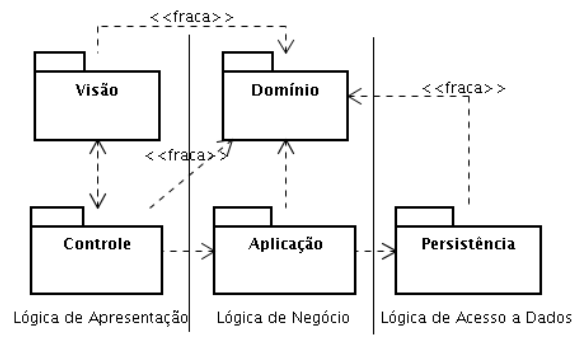
\includegraphics[scale=.6]{figuras/fig-ref-service-layer} 
	\caption{Arquitetura padrão para WIS baseada no padrão arquitetônico \textit{Service Layer}~\cite{fowler:peaa02}.}
	\label{fig-ref-service-layer}
\end{figure}

\begin{itemize}

	\item \textbf{Lógica de Apresentação:} possui a responsabilidade de realizar a interação entre o sistema e o usuário, exibindo as informações e interpretando os comandos em ações da persistência de dados e da lógica de negócio.
		
		\subitem -- Pacote de \textbf{Visão:} realiza a iteração humano-computador, definindo o formato de relatórios, formulários e janelas, sendo que a construção de protótipos é muito útil para facilitar o desenvolvimento dos mecanismos que serão utilizados. 
		
		\subitem -- Pacote de \textbf{Controle:} define as classes que serão responsáveis por controlar a iteração, enviando requisições para os objetos da Lógica de Negócio.  
	
	\item \textbf{Lógica de Negócio:} engloba as funcionalidades que dão suporte aos processos de negócio, concentrando as regras de negócio, conceitos do domínio, cálculos e processamentos.
	
		\subitem -- Pacote de \textbf{Domínio:} reúne o relacionamento direto entre os diagramas de classes produzidos na fase de análise e os conceitos do domínio do problema. 
		
		\subitem -- Pacote de \textbf{Aplicação:} está ligado ao modelo de casos de uso e é projetado de maneira independente da interface com o usuário.
	
	\item \textbf{Lógica de Acesso a Dados:} estabelece o acesso a dados, gerenciando requisições e cuidando da sincronização de elementos de dados.
	
		\subitem -- Pacote de \textbf{Persistência:} contém as classes que são responsáveis por gravar os objetos de domínio que necessitam ser persistidos pelo sistema em um banco de dados. O método FrameWeb sugere que as classes sigam o padrão de projeto \textit{Data Access Object} (DAO)~\cite{alur-et-al:bpds03}. Este padrão determina uma interface de operações de persistência, incluindo métodos para a criação, recuperação, alteração e exclusão, agrupando o código relacionado à entidade persistente~\cite{bauer-et-al:jpwh07}. 

\end{itemize}

\subsection{Linguagem de Modelagem}
\label{sec-ref-linguagem-modelagem}

Com o objetivo de representar de maneira direta os conceitos existentes nos \textit{frameworks} que podem ser integrados, o uso de uma linguagem específica de modelagem se tornou necessária~\cite{martins-souza:webmedia15}, pois os artefatos que serão codificados pelos desenvolvedores após a fase de projeto também devem ser modelados. O FrameWeb apresenta uma linguagem de modelagem que estende o meta-modelo UML, representando os componentes relacionados aos \textit{frameworks} e os componentes mais utilizados no desenvolvimento \textit{Web}. Um perfil UML é utilizado para a construção de quatro tipos de diagramas: 

\begin{itemize}  

	\item \textbf{Modelo de Entidades:} partindo do modelo de classes desenvolvido na fase de análise, os objetos de domínio do problema que serão persistidos no banco de dados são representados por um diagrama de classes da UML. Além disso, os mapeamentos que guiam a persistência dos objetos destas classes são adicionados;
	
	\item \textbf{Modelo de Persistência:} um diagrama de classes da UML representa a implementação das classes DAO existentes no sistema e que serão persistidas, exibindo todas as implementações das interfaces, assim como os seus respectivos métodos;
	
	\item \textbf{Modelo de Navegação:} demonstra as páginas \textit{Web} do sistema, seus atributos e suas iterações, exibindo o funcionamento dos inúmeros componentes que formam a camada de Lógica de Apresentação;
	
	\item \textbf{Modelo de Aplicação:} exibe através de um diagrama de classes da UML, as classes de serviço, que implementam os casos de uso e as suas dependências.

\end{itemize}

A definição da linguagem de modelagem permite, ainda, a criação de ferramentas de apoio ao método, como um editor gráfico~\cite{campos-souza:webmedia17} e um gerador de código~\cite{almeida-et-al:webmedia17}.



\section{Frameworks}
\label{sec-ref-frameworks}

Para realizar a implementação de um WIS, através da Engenharia \textit{Web}, o que mais se pode encontrar são ferramentas, propostas de metodologias e inúmeras linguagens que facilitam o processo realizado pelos desenvolvedores. Após a construção dos primeiros sistemas, verificou-se que os WISs possuíam uma infraestrutura arquitetônica bem parecida. Desta maneira, diversos \textit{frameworks} foram criados para generalizar essa infraestrutura e para facilitar a realização do desenvolvimento de novas aplicações.

Assim, um \textit{framework} pode ser considerado um design reutilizável de uma parte ou de todo o sistema, sendo representado por um conjunto de classes abstratas e concretas que demonstram a forma como suas instâncias interagem com um grande potencial de especialização~\cite{mattsson-et-al:csef99}. Com a utilização das funcionalidades que os \textit{frameworks} oferecem, a implementação dos códigos fontes das aplicações se tornam bem mais simples, minimizando os custos e o tempo utilizado.

Diversos \textit{frameworks} foram criados para a plataforma Java e após a construção de inúmeros WISs, \citeonline{souza:masterthesis07} estabeleceu uma organização para os \textit{frameworks} em seis categorias diferentes:    

\begin{itemize} 
	
	\item \textit{Frameworks} MVC (Controladores Frontais);
	
	\item \textit{Frameworks} Decoradores;
	
	\item \textit{Frameworks} de Mapeamento Objeto/Relacional;
	
	\item \textit{Frameworks} de Injeção de Dependência (Inversão de Controle);
	
	\item \textit{Frameworks} para Programação Orientada a Aspectos (AOP);
	
	\item \textit{Frameworks} para Autenticação e Autorização.
   
\end{itemize}

O \textit{framework} Grails utilizado neste trabalho, pertence à categoria de \textit{frameworks} MVC (Controladores Frontais) e será descrito nas próximas subseções.

\subsection{Controladores Frontais: Frameworks MVC}
\label{sec-ref-framework-mvc}

O padrão MVC, abreviatura de Modelo-Visão-Controlador (\textit{Model-View-Controller}), possibilita a divisão do projeto em camadas muito bem definidas. Correspondendo a objetos da camada de Lógica de Negócio, o \textbf{(modelo)} faz referência aos objetos que descrevem as informações sobre o negócio. A \textbf{(visão)} cuida da exibição e da entrada de informações na interface do usuário. O \textbf{(controlador)} trata das requisições, envia para a camada de Lógica de Negócio e após receber as respostas, realiza a solicitação para que as informações sejam atualizadas pela \textbf{(visão)}. A Figura~\ref{fig-ref-mvc} demonstra como funciona esse padrão arquitetural.  

\begin{figure}[h]
	\centering
	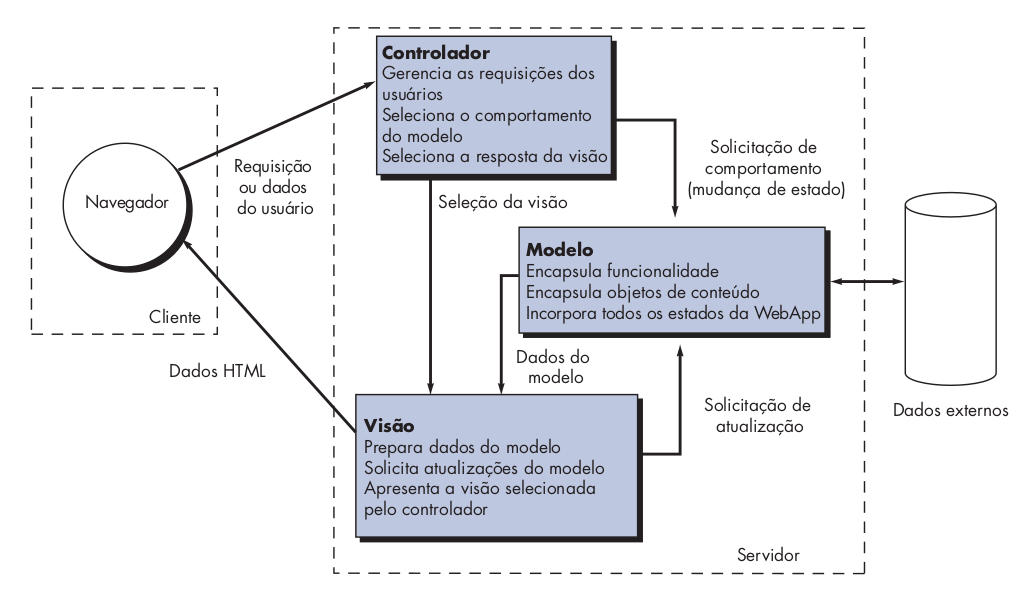
\includegraphics[scale=.45]{figuras/fig-ref-mvc} 
	\caption{Arquitetura MVC através de uma representação esquemática~\cite{pressman:es11}.}
	\label{fig-ref-mvc}
\end{figure}

O \textbf{(modelo)} apenas tem conhecimento sobre a lógica e os dados que estão armazenados no sistema através de bancos de dados ou arquivos. Ele é considerado o núcleo da aplicação e é onde as operações de CRUD podem ser realizadas. A \textbf{(visão)} não possui lógica de negócio e fica responsável por controlar a entrada dos dados fornecidos pelo usuário, devolvendo a saída das informações assim que elas forem repassadas pelo \textbf{(controlador)}. O \textbf{(controlador)} funciona como um intermediário, organizando os eventos enviados pela interface do usuário e os direcionando para o \textbf{(modelo)}.

O padrão MVC aborda dois tipos de separação. No primeiro tipo, existe uma separação entre a apresentação \textbf{(visão)} e a lógica de negócio \textbf{(modelo)}. No segundo tipo, o \textbf{(controlador)} é separado da \textbf{(visão)}, sendo este segundo tipo menos importante do que o primeiro. Como inúmeros sistemas possuem um único controlador por visão, o segundo tipo quase não é utilizado. Entretanto, o segundo tipo é mais comum em interfaces \textit{Web}, pois a parte de \textbf{(visão)} \textit{front end} é naturalmente separada do \textbf{(controlador)}~\cite{fowler:peaa02}.

De acordo com \citeonline{souza:masterthesis07}, a arquitetura MVC necessita de algumas alterações para atender as necessidades dos aplicativos \textit{Web}. O \textbf{(modelo)}, situado no servidor \textit{Web}, não consegue enviar as notificações das alterações para a \textbf{(visão)}, já que se encontra no navegador do lado do cliente e a comunicação é sempre iniciada pelo cliente. Então, apesar de MVC ser um nome bem conceituado, o nome correto para esse padrão arquitetônico, quando aplicado à \textit{Web}, seria ``Controlador Frontal'' (\textit{Front Controller})~\cite{alur-et-al:bpds03}. O padrão Controlador Frontal pode ser visualizado na Figura~\ref{fig-ref-controlador-frontal}.   

\begin{figure}[h]
	\centering
	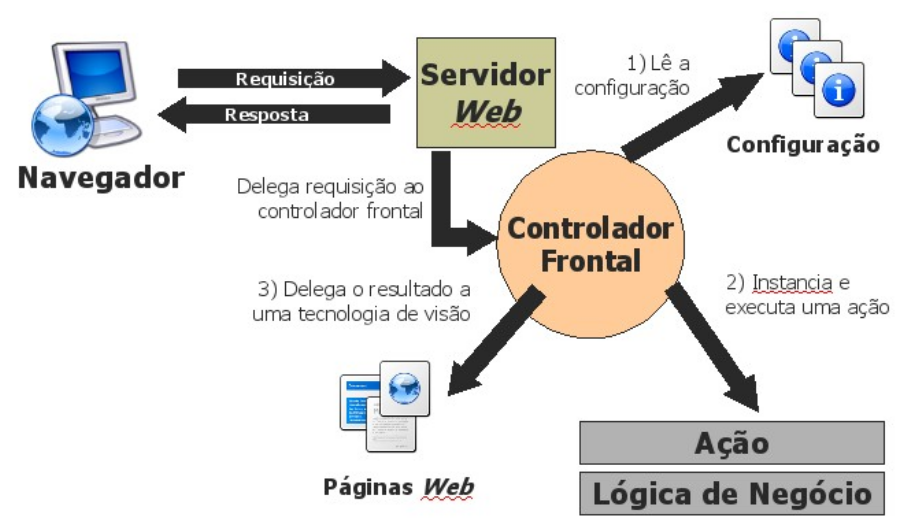
\includegraphics[scale=.45]{figuras/fig-ref-controlador-frontal} 
	\caption{Funcionamento do padrão arquitetônico Controlador Frontal na \textit{Web}~\cite{souza:masterthesis07}.}
	\label{fig-ref-controlador-frontal}
\end{figure}

\subsection{Framework Grails}
\label{sec-ref-framework-grails}

O Grails é um \textit{framework} voltado para o desenvolvimento de aplicações \textit{web}, baseado em MVC e que utiliza a linguagem Groovy. Com o objetivo de facilitar a vida dos desenvolvedores, a partir da utilização do Grails, a implementação da lógica de negócio passou a ser realizada de maneira imediata e sem a preocupação com a integração de inúmeras bibliotecas, como o Hibernate para a persistência, Spring e várias outras.

Visualizar de maneira instantânea o resultado das alterações em tempo de execução, também é uma característica do Grails. Algumas outras particularidades também podem ser mencionadas: as camadas de visualização e controle baseadas nas classes de domínio podem ser geradas automaticamente, a inversão de controle e a injeção de dependências são baseadas em Spring, os principais \textit{frameworks} e bibliotecas Java podem ser integrados facilmente e o \textit{framework} para persistência GORM fica responsável por controlar a validação dos dados, tirando a preocupação dos desenvolvedores com arquivos de mapeamento ou com anotações.

Após o projeto utilizando o \textit{framework} Grails ser finalizado, é possível obter como resultado uma aplicação Java EE completa, possuindo escalabilidade, robustez, desempenho e alta disponibilidade. Além disso, Grails é altamente portável entre servidores de aplicação~\cite{weissmann:fgapdw15}.       


\subsection{Linguagem Groovy}
\label{sec-ref-linguagem-groovy}


Alterar o comportamento do código enquanto ele é executado pode ser bem simples utilizando Groovy. Por se tratar de uma linguagem dinâmica e orientada a objetos, ela tem como vantagem a execução de tarefas em tempo de execução, se destacando com relação as outras linguagens que só executam através de padrões de projetos ou no momento da compilação. A linguagem Groovy é altamente compatível com os códigos desenvolvidos através da linguagem Java, que podem ser acessados transparentemente pelos códigos implementados em Groovy e vice-versa.

Com relação às variáveis que são utilizadas na linguagem, a definição dos tipos pode acontecer de modo estático ou dinamicamente, ou seja, a definição dos tipos das variáveis utilizadas no Groovy não é obrigatório. Os métodos são bem mais simples de serem definidos, pois não é preciso explicitar o tipo de retorno e nem utilizar a instrução return para retornar um valor.

No decorrer do Capítulo~\ref{sec-projeto} serão abordados mais alguns detalhes referentes a linguagem Groovy, que serão exemplificados de acordo como a demonstração da implementação do projeto.         



       
% ==============================================================================
% TCC - Nome do Aluno
% Capítulo 3 - Especificação de Requisitos
% ==============================================================================
\chapter{Especificação de Requisitos e Análise do SCAP}
\label{sec-requisitos}

Este capítulo apresenta uma descrição de escopo referente ao SCAP (Sistema de Controle de Afastamento de Professores), assim como o modelo de casos de uso e o diagrama de classes que foi levantado anteriormente por~\citeonline{duarte-pg14} e posteriormente analisado por~\citeonline{prado-pg15}. 

\section{Descrição do Escopo}
\label{sec-requisitos-descricao-escopo}

O SCAP surgiu com o objetivo de auxiliar o Departamento de Informática (DI) da UFES no controle e no registro de solicitações de afastamento do seus professores, para que eles possam participar de eventos que acontecem no Brasil e no exterior. Essas solicitações de afastamento necessitam passar por uma série de avaliações para que sejam aprovadas. Elas são avaliadas pelos professores do DI e dependendo do caso, também devem ser avaliadas pelo Centro Tecnológico (CT) e pela Pró-Reitoria de Pesquisa e Pós-Graduação (PRPPG). Nestes casos, somente após receber a aprovação de todas as instâncias, o afastamento é publicado no Diário Oficial da União e o professor recebe a autorização para participar do evento.     

A Câmara Departamental (composta pelos representantes discentes e pelos funcionários do departamento) fica responsável por avaliar e aprovar as solicitações de afastamento para eventos no Brasil. O chefe do departamento (cargo ocupado por um professor do DI através de um mandato temporário) recebe a solicitação de afastamento pelo email e após dez dias, se nenhum membro da Câmara Departamental for contra ao pedido, o afastamento é aprovado. Assim, para eventos nacionais, o processo permanece dentro do DI.

Para pedidos de afastamento referente a eventos internacionais, um professor (sem parentesco com o solicitante) é escolhido para se tornar relator do pedido. Assim que o relator manda o parecer, o pedido passa por avaliação para aprovação como no caso descrito com eventos que são realizados no Brasil. Para que o pedido seja publicado no Diário Oficial da União, ele deve receber a aprovação do CT e da PRPPG. Entretanto, o SCAP não possui uma integração com os processos do CT e da PRPPG, fazendo com que o controle das tramitações permaneça dentro do DI, restringindo o escopo do sistema.

Com o intuito de automatizar as tramitações das solicitações de afastamento, o SCAP auxilia os professores e secretários do DI, facilitando o processo desde a criação até a aprovação e armazenamento. Com o envio de e-mails automáticos para os envolvidos e com a utilização de formulários para a criação dos documentos necessários, o sistema pode ser considerado fundamental para esse processo.      

\section{Modelo de Casos de Uso}
\label{sec-requisitos-modelo-casos-uso}

Após o levantamento de requisitos e da definição do escopo, os atores identificados no sistema SCAP são apresentados na Tabela~\ref{tabela-atores-scap}.  

\begin{table}[h]
	\centering	
	\vspace{0.5cm}
	\footnotesize
	\caption{Atores do SCAP~\cite{duarte-pg14}.}	
	\label{tabela-atores-scap}
	\begin{tabular}{|p{5.0cm}|p{9.0cm}|}  \hline 
 		
 		\rowcolor[rgb]{0.8,0.8,0.8} \textbf{Ator} & \textbf{Descrição} \\\hline 
		
		\textbf{Professor} & Professores efetivos do DI/UFES. \\\hline
		
		\textbf{Chefe do Departamento} & Professores do DI/UFES que estão realizando a função administrativa de chefe e subchefe do departamento. \\\hline
		
		\textbf{Secretário} & Secretário do DI/UFES. \\\hline
		
	\end{tabular}
\end{table}

A parte administrativa do sistema fica por conta dos \textbf{secretários}. Eles possuem a responsabilidade de realizar o cadastro dos mandatos dos chefes do departamento, realizar o cadastro dos professores e dos seus respectivos parentescos. Quando surgem pareceres de fora do DI e quando os pedidos de afastamento são finalizados, os \textbf{secretários} também ficam responsáveis pelo controle dessas tarefas.

O SCAP fornece algumas funcionalidades para os \textbf{professores}. Eles podem realizar o cadastro das solicitações de afastamento e realizar uma manifestação contra o afastamento de outro professor, caso ainda esteja dentro do prazo. Além disso, o \textbf{professor} fica responsável por recomendar a aprovação ou não de um afastamento no exterior, caso ele seja adicionado como relator do mesmo. 

Se um \textbf{professor} se tornar \textbf{chefe do departamento} através de um mandato, ele deve realizar o encaminhamento de solicitações aos relatores que farão o deferimento de pareceres com relação aos afastamentos internacionais.

O diagrama de casos de uso do SCAP pode ser visualizado através da Figura~\ref{fig-requisitos-casos-uso}. Uma pequena descrição dos casos de uso será apresentada nos próximos parágrafos e uma versão mais completa dessa descrição pode ser encontrada em~\cite{duarte-pg14,prado-pg15}.
     
\begin{figure}[h]
	\centering
	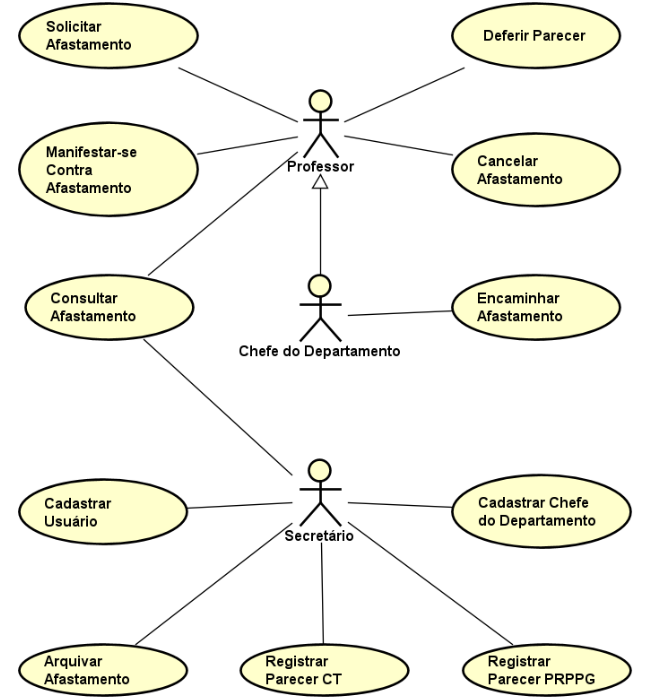
\includegraphics[scale=0.5]{figuras/fig-requisitos-casos-uso} 
	\caption{Diagrama de Casos de Uso do SCAP.}
	\label{fig-requisitos-casos-uso}
\end{figure}

No sistema, um professor realiza o cadastro de um pedido de afastamento por meio do caso de uso \textbf{Solicitar Afastamento}, fornecendo todos os dados que são necessários para realizar a tramitação. Um professor pode cancelar uma solicitação de afastamento utilizando o caso de uso \textbf{Cancelar Afastamento}, realizando a alteração do status para cancelado.

Após escolher um relator para um pedido de afastamento internacional, o Chefe do Departamento pode executar o caso de uso \textbf{Encaminhar Afastamento}. Quando um professor que se tornou relator através da indicação do Chefe do Departamento realizar o cadastro do seu parecer sobre o afastamento, o caso de uso \textbf{Deferir Parecer} pode ser utilizado.

Um professor, um chefe de departamento ou um secretário podem utilizar o caso de uso \textbf{Consultar Afastamento} assim que necessitarem obter informações sobre uma solicitação de afastamento. Se um professor for contra a um pedido de afastamento, o caso de uso \textbf{Manifestar-se Contra Afastamento} pode ser utilizado e após o motivo ser cadastrado, uma reunião é agendada para decidir a aprovação ou reprovação da solicitação.

Um secretário realiza o cadastramento de novos professores ou secretários através do caso de uso \textbf{Cadastrar Usuário}, onde são informados todos os dados necessários. Um secretário também utiliza o caso de uso \textbf{Cadastrar Chefe do Departamento} para especificar o período do mandato do novo chefe do departamento.
  
Quando existe uma solicitação de afastamento internacional, um secretário realiza o cadastro do parecer do Centro Tecnológico e da Pró-Reitoria de Pesquisa e Pós-Graduação por meio dos casos de uso \textbf{Registrar Parecer CT} e \textbf{Registrar Parecer PRPPG}.

O caso de uso \textbf{Arquivar Afastamento} é executado após a tramitação de uma solicitação de afastamento ser realizada, fazendo com que um secretário realize a alteração do status para ``Arquivado''.   

\section{Análise do SCAP}
\label{sec-requisitos-analise-scap}

O diagrama de classes do SCAP pode ser visualizado através da Figura~\ref{fig-requisitos-diagrama-classes}. As instâncias das classes são especificadas de acordo com o comportamento exercido pelos objetos que seguem as especificações das classes. 

\begin{figure}[h]
	\centering
	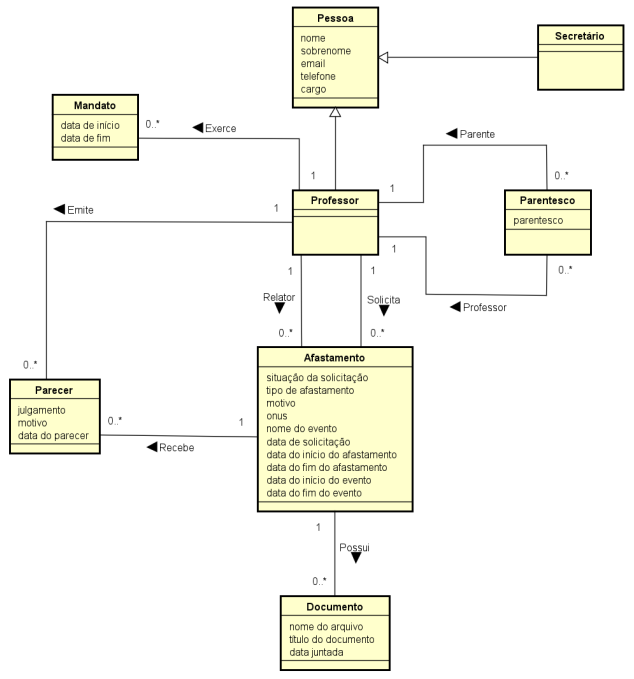
\includegraphics[scale=0.7]{figuras/fig-requisitos-diagrama-classes} 
	\caption{Diagrama de Classes do SCAP.}
	\label{fig-requisitos-diagrama-classes}
\end{figure}

Herdando todos os atributos da classe \textbf{Pessoa}, os professores são representados pela classe \textbf{Professor} e os secretários são representados pela classe \textbf{Secretário}. Os professores podem possuir relações de parentesco, seja ela matrimonial ou sanguínea. Essas relações são representadas pela classe \textbf{Parentesco}. Um professor pode ocupar o cargo de chefe ou subchefe do departamento, sendo que o tempo de permanência no cargo é representado pela classe \textbf{Mandato}.

Os pedidos de afastamento solicitados por professores são representados pela classe \textbf{Afastamento}. Nela se encontram todas as informações necessárias para realizar as tramitações. Esta classe pode conter documentos que são visualizados através da classe \textbf{Documento}. Quando um pedido de afastamento se trata de um evento internacional, a classe \textbf{Relator} deve ser utilizada informando o professor que foi indicado para isso.

A classe \textbf{Parecer} é utilizada quando um professor efetua a emissão de um parecer com relação a um afastamento. Um professor pode se tornar relator e criar pareceres de vários afastamentos diferentes. 

Restrições de integridade do sistema foram identificadas por \citeonline{duarte-pg14} e, após concluir a implementação de uma nova versão, \citeonline{prado-pg15} sentiu a necessidade de adicionar novas restrições. As restrições de integridade do SCAP que foram atualizadas estão descritas a seguir:
 
\begin{itemize}

	\item Um professor não pode ser relator de um afastamento solicitado por um parente;
	
	\item O secretário do departamento não pode abrir uma solicitação de afastamento;
	
	\item Não pode haver mais de dois professores (chefe e subchefe de departamento) exercendo um mandato ao mesmo tempo;
	
	\item A data de início de um mandato de professor não pode ser posterior a data de fim do mesmo mandato;
	
	\item A data de início de um afastamento não pode ser posterior a data de fim do mesmo afastamento;
	
	\item Um professor não pode ser solicitado para dar um parecer sobre sua própria solicitação de afastamento. 
   
\end{itemize} 

% ==============================================================================
% TCC - Nome do Aluno
% Capítulo 4 - Projeto Arquitetural e Implementação
% ==============================================================================
\chapter{Projeto Arquitetural e Implementação}
\label{sec-projeto}

De acordo com o que já foi mencionado anteriormente, o método FrameWeb oferece suporte a quatro categorias de \textit{frameworks}: Controlador Frontal, Injeção de Dependências, Mapeamento Objeto/Relacional e Segurança. Por este motivo, a aplicação do método na fase de projeto vem sendo testada através da implementação do sistema SCAP, utilizando \textit{frameworks} que fazem parte destas categorias.

Como o objetivo principal deste trabalho era verificar os resultados da aplicação e testar a eficácia do método FrameWeb, a ferramenta SCAP não necessitou ser entregue englobando todas as suas funcionalidades. Assim, algumas restrições de integridade não foram implementadas, a ferramenta não possui a funcionalidade de enviar emails, gerar atas de reuniões e nem anexar documentos.

Neste capítulo, através da Seção~\ref{sec-projeto-arquitetura-sistema}, é descrito como o \textit{framework} Grails organiza os diretórios do projeto. A Seção~\ref{sec-projeto-tecnologias-presentes} apresenta as tecnologias presentes no projeto através do uso do \textit{framework} Grails. A Seção~\ref{sec-projeto-modelos-frameweb} demonstra os modelos gerados por meio da aplicação do método FrameWeb e a Seção~\ref{sec-projeto-exibicao-sistema}, exibe as telas do sistema SCAP que foi implementado por meio do \textit{framework} Grails.           

\section{Arquitetura do Sistema}
\label{sec-projeto-arquitetura-sistema}

De uma maneira simplificada, a arquitetura do sistema é a organização ou a estrutura de componentes de programa, a maneira como esses componentes realizam iterações e a estrutura de dados que são utilizadas por estes componentes. De uma forma mais abrangente, entretanto, os componentes podem ser generalizados para representar as suas iterações e os principais elementos de um sistema~\cite{pressman:es11}.

A Figura~\ref{fig-projeto-estrutura-grails} demonstra a estrutura da hierarquia dos diretórios e arquivos que são criados através do \textit{framework} Grails.

\begin{figure}[!h]
	\centering
	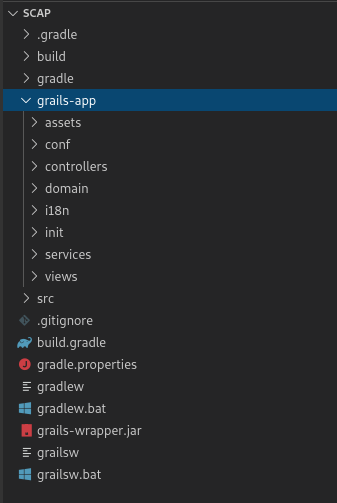
\includegraphics[scale=0.7]{figuras/fig-projeto-estrutura-grails} 
	\caption{Estrutura criada pelo \textit{framework} Grails.}
	\label{fig-projeto-estrutura-grails}
\end{figure}

Por meio dos relatos apresentados por~\citeonline{beder:ew12}, a hierarquia de diretórios e arquivos do \textit{framework} Grails segue o paradigma \textbf{\textit{Convention Over Configuration} (CoC)}. O uso do \textbf{CoC} tem como objetivo diminuir a quantidade de decisões tomadas pelos desenvolvedores, adotando como ``padrão'' algo que é utilizado de forma comum, uma convenção. Seguindo as convenções, os desenvolvedores já sabem a priori onde se encontram todos os elementos que compõem a aplicação em desenvolvimento.

Na lista abaixo são apresentados de maneira geral os diretórios criados através do \textit{framework} Grails. As abas dos diretórios estão representadas em negrito:

\begin{itemize}

	\item \textbf{``grails-app/assets'':} local onde se encontram os arquivos de imagens, javascript e \textit{stylesheets};

	\item \textbf{``grails-app/conf'':} local onde se encontram as configurações da aplicação, tais como a configuração do banco, as configurações de inicialização, entre outros;

	\item \textbf{``grail-app/controllers'':} local onde ficam localizados todos os controladores criados;
	
	\item \textbf{``grails-app/domain'':} local onde se encontram os modelos ou classes de domínio;
	
	\item \textbf{``grails-app/i18n'':} local onde são armazenados os pacotes de mensagens relacionados à internacionalização;
	
	\item \textbf{``grails-app/services'':} local onde se encontram as classes utilizadas na camada de serviços (\textit{Web Services});
	
	\item \textbf{``grails-app/views'':} local onde estão localizadas as visões, ou seja, os arquivos GSP (\textit{Groovy Server Pages}), que são responsáveis por renderizar as páginas utilizadas pela aplicação. 
	
\end{itemize}

Dentro dos diretórios, ainda é possível incluir arquivos referentes a bibliotecas terceirizadas que podem ser utilizadas no projeto, assim como códigos fontes escritos na linguagem Java ou na linguagem Groovy. Estes códigos podem ser reaproveitados pela aplicação.

\section{Tecnologias Presentes no Projeto}
\label{sec-projeto-tecnologias-presentes}

Utilizando o \textit{framework} Grails, esta versão do SCAP foi implementada na linguagem Apache Groovy. Os dados armazenados no banco de dados necessitavam estar de acordo com as especificações dos modelos utilizados no projeto. Para que essa tarefa fosse monitorada, foi utilizado a ferramenta phpMyAdmin, que facilitou a visualização e conferência dos dados.

Descrevendo mais sobre a linguagem Groovy, ela também pode ser utilizada como uma linguagem de \textit{script}, não sendo necessário realizar a geração de arquivos executáveis e nem a sua compilação. O Groovy simplifica a implementação, adicionando dinamicamente às suas classes os métodos de acesso (\textit{gets} e \textit{sets}), economizando esforço e tempo. Com o objetivo de simplificar a sintaxe da linguagem Java, o Groovy representa comportamentos dinâmicos, como escritas e leituras, consulta a banco de dados e geração de objetos em tempo de execução ao invés de compilação~\cite{konig-et-al:gia07}.

Nas subseções abaixo estão descritas mais algumas tecnologias que foram utilizadas no projeto através do \textit{framework} Grails.

\subsection{Scaffolding}
\label{sec-projeto-scaffolding}

A abordagem Scaffolding é um termo que foi adotado pelo \textit{framework} Grails para realizar a geração dos controladores e das visões relacionadas às classes de domínio. Através dele, é possível gerar todo o código responsável por fornecer um CRUD essencial para o sistema, permitindo incluir, ler, atualizar e deletar os registros armazenados no banco de dados. Ainda é possível criar códigos de autenticação/autorização, testes unitários, entre outras operações~\cite{beder:ew12}.

De acordo com~\citeonline{beder:ew12}, o Scaffolding pode ser estático ou dinâmico. O Scaffolding estático produz, através da utilização de \textit{templates}, o código relacionado as visões e aos controladores que podem receber personalizações das equipes de desenvolvedores \textit{web}. Já o Scaffolding dinâmico pode servir a vários propósitos, como na criação de interfaces simples, sem o intuito de realizar muitas personalizações nas visões que são geradas em tempo de execução. Para a implementação desta versão do SCAP, foi utilizado o Scaffolding dinâmico.   

\subsection{Gradle}
\label{sec-projeto-gradle}

O Gradle é uma ferramenta de construção de \textit{build} bastante poderosa que pode ser utilizada na gerência de projetos, gestão de dependências, padronização de diretórios, construção, ciclo de vida, entre outras funcionalidades. O Gradle ainda possui uma quantidade imensa de \textit{plug-ins} que podem ser muito aproveitosos nos projetos~\cite{weissmann:fgapdw15}.

Com a adoção do Gradle pelo \textit{framework} Grails, foi necessário realizar algumas mudanças na localização de alguns diretórios e de alguns arquivos com relação às versões anteriores. Isso facilitou o entendimento da estrutura e a configuração dos arquivos existentes.

\subsection{GORM}
\label{sec-projeto-gorm}

O GORM (\textit{Grails Object Relational Mapping}) é uma poderosa API (\textit{Application Programming Interface}) que facilita muito a execução de tarefas relacionadas à persistência de objetos. Nas versões iniciais do \textit{framework} Grails, o GORM era basicamente uma fina camada de código Groovy sobre o Hibernate, que fornecia uma interface de programação onde era possível aproveitar as características dinâmicas da linguagem~\cite{weissmann:fgapdw15}.

De acordo com~\citeonline{weissmann:fgapdw15}, hoje em dia, o GORM passou a ser visto como uma API de persistência Groovy real, onde é possível desenvolver sistemas em Grails que usem qualquer tipo de SGBD (Sistema Gerenciador de Banco de Dados), relacional ou não. Para isto, é necessário que seja escrita uma implementação do GORM para o SGDB que será utilizado. Uma observação interessante é que o GORM também pode ser utilizado com sucesso independentemente do Grails.  

\section{Modelos FrameWeb}
\label{sec-projeto-modelos-frameweb}

Nas subseções a seguir são descritos e apresentados os modelos referentes à aplicação do método FrameWeb que foi realizada durante a fase de projeto arquitetural do SCAP. A ferramenta FrameWeb Editor~\cite{campos-souza:webmedia17} foi utilizada para realizar a criação dos quatro tipos básicos de modelos FrameWeb, pois ela oferece um ferramental bem conhecido em softwares de modelagem contendo características e propriedades próprias da linguagem.  

\subsection{Modelo de Navegação}
\label{sec-projeto-modelo-navegacao}

Os Modelos de Navegação foram gerados de acordo com os casos de uso do sistema. A Figura~\ref{fig-projeto-cadastrarUsuarioProfessor} e a Figura~\ref{fig-projeto-cadastrarUsuarioSecretario} representam o caso de uso ``Cadastrar Usuário'', que é realizado por um secretário. O caso de uso ``Cadastrar Chefe do Departamento'' também é utilizado por um secretário e foi representado através da Figura~\ref{fig-projeto-cadastrarChefeDepartamento}. 

\begin{figure}[!h]
	\centering
	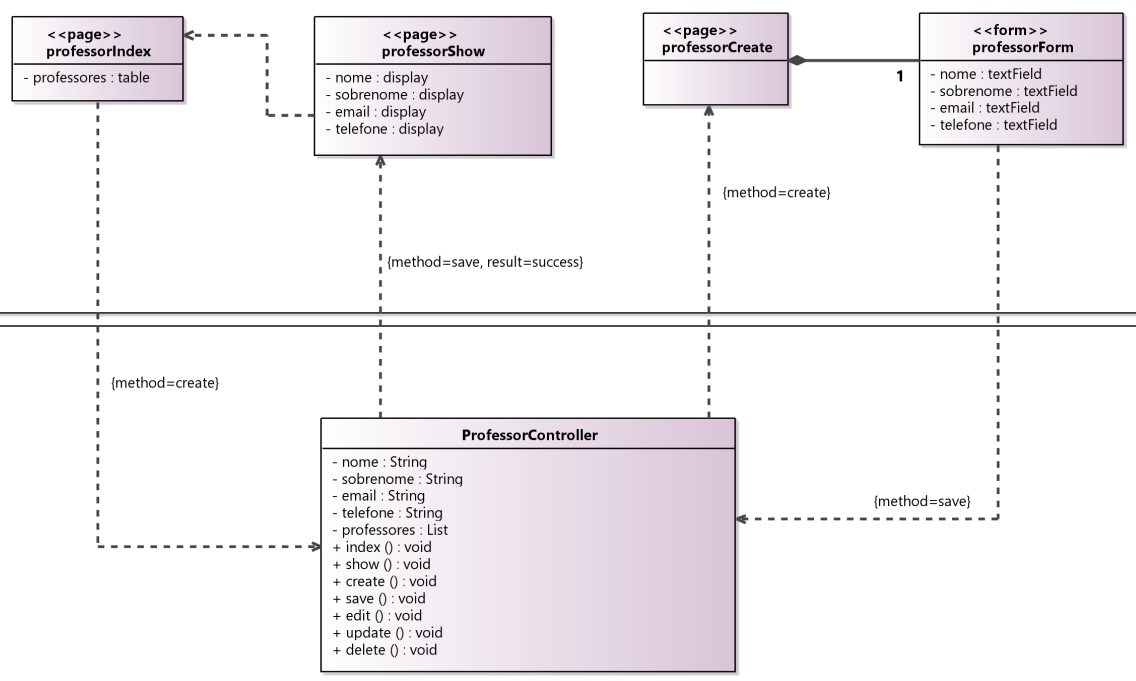
\includegraphics[width=1\textwidth]{figuras/fig-projeto-cadastrarUsuarioProfessor.png}
	\caption{Modelo de Navegação do Caso de Uso: Cadastrar Usuário - Professor.}
	\label{fig-projeto-cadastrarUsuarioProfessor}
\end{figure}

\begin{figure}[!h]
	\centering
	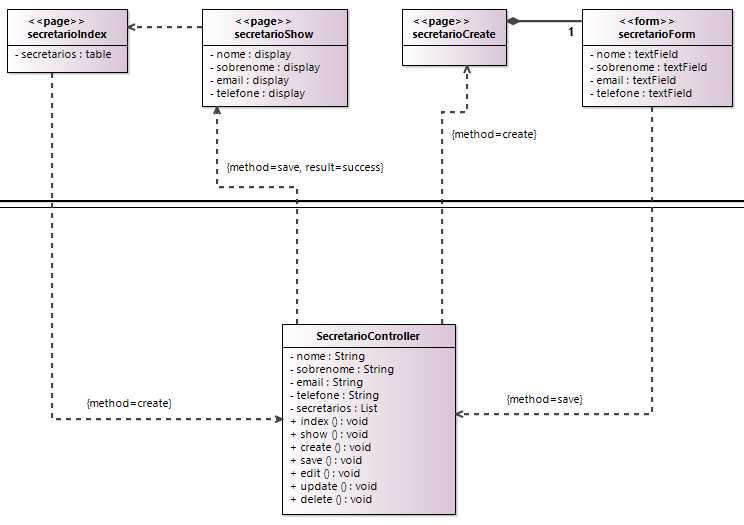
\includegraphics[width=1\textwidth]{figuras/fig-projeto-cadastrarUsuarioSecretario.png}
	\caption{Modelo de Navegação do Caso de Uso: Cadastrar Usuário - Secretário.}
	\label{fig-projeto-cadastrarUsuarioSecretario}
\end{figure}

\begin{figure}[!h]
	\centering
	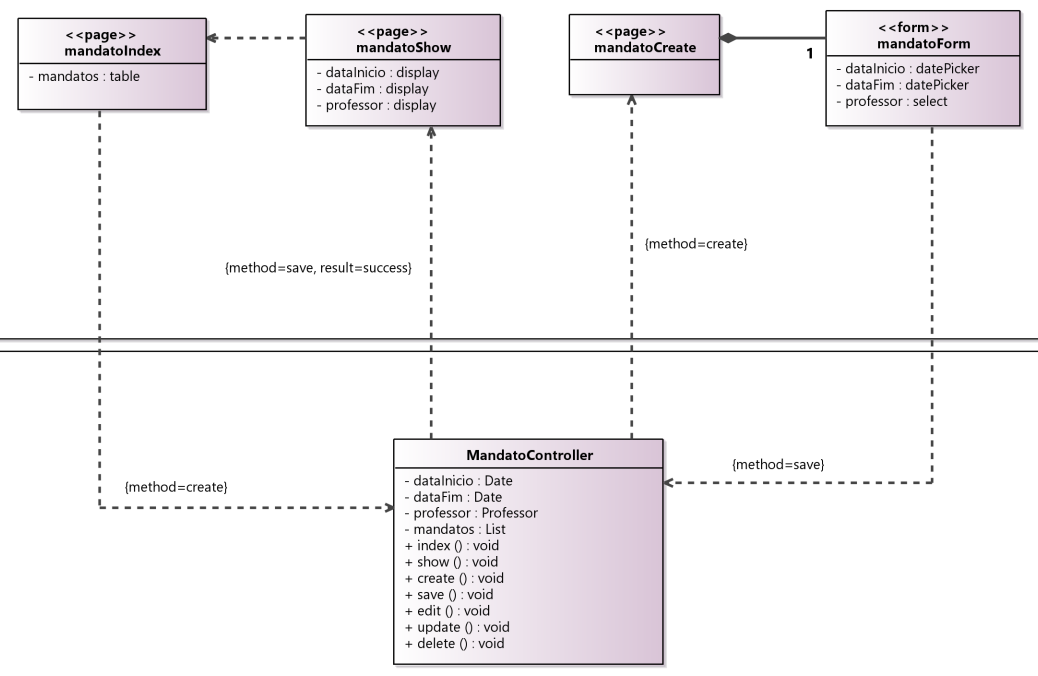
\includegraphics[width=1\textwidth]{figuras/fig-projeto-cadastrarChefeDepartamento.png}
	\caption{Modelo de Navegação do Caso de Uso: Cadastrar Chefe do Departamento.}
	\label{fig-projeto-cadastrarChefeDepartamento}
\end{figure}

A Figura~\ref{fig-projeto-solicitarAfastamento} representa o caso de uso ``Solicitar Afastamento'', que acontece quando um professor realiza o cadastro de um pedido de afastamento. Caso exista um pedido de afastamento internacional, o chefe do departamento utiliza o caso de uso ``Encaminhar Afastamento'', que pode ser visualizado na Figura~\ref{fig-projeto-encaminharAfastamento}. 

\begin{figure}[!h]
	\centering
	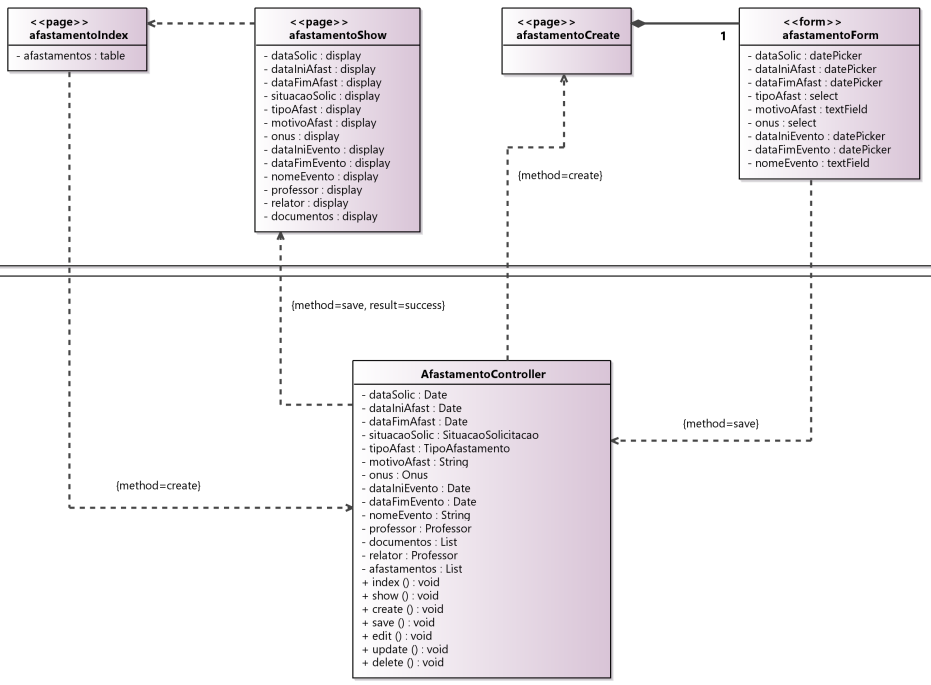
\includegraphics[width=1\textwidth]{figuras/fig-projeto-solicitarAfastamento.png}
	\caption{Modelo de Navegação do Caso de Uso: Solicitar Afastamento.}
	\label{fig-projeto-solicitarAfastamento}
\end{figure}

\begin{figure}[!h]
	\centering
	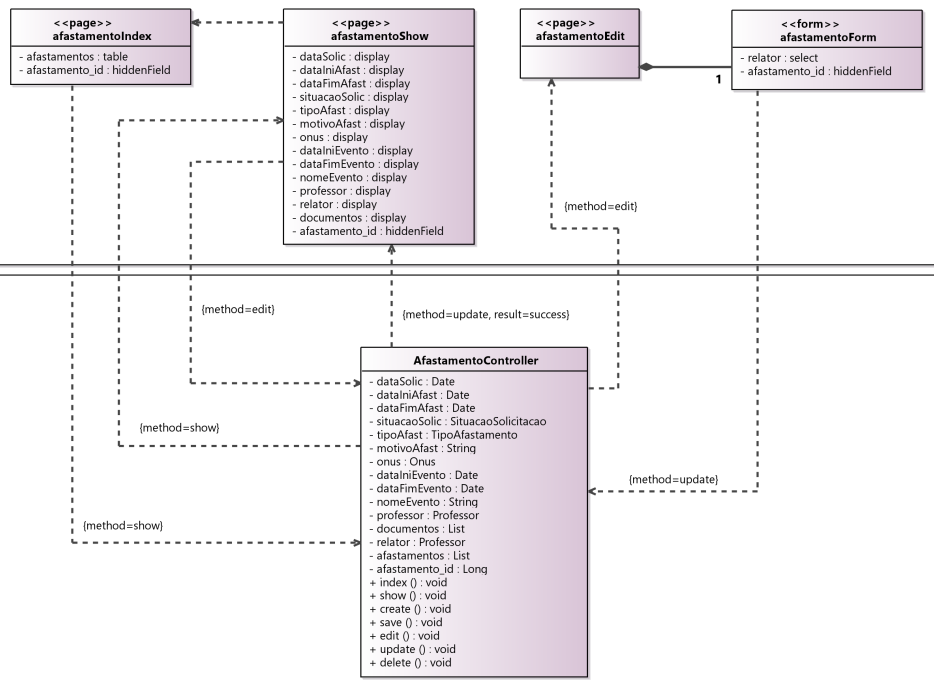
\includegraphics[width=1\textwidth]{figuras/fig-projeto-encaminharAfastamento.png}
	\caption{Modelo de Navegação do Caso de Uso: Encaminhar Afastamento.}
	\label{fig-projeto-encaminharAfastamento}
\end{figure}

Os casos de uso ``Deferir Parecer'' e ``Manifestar-se Contra Afastamento'' são bem parecidos, pois é necessário realizar o cadastro de um parecer. Portanto, eles foram representados através da Figura~\ref{fig-projeto-defParecer_manifContra}. 

\begin{figure}[!h]
	\centering
	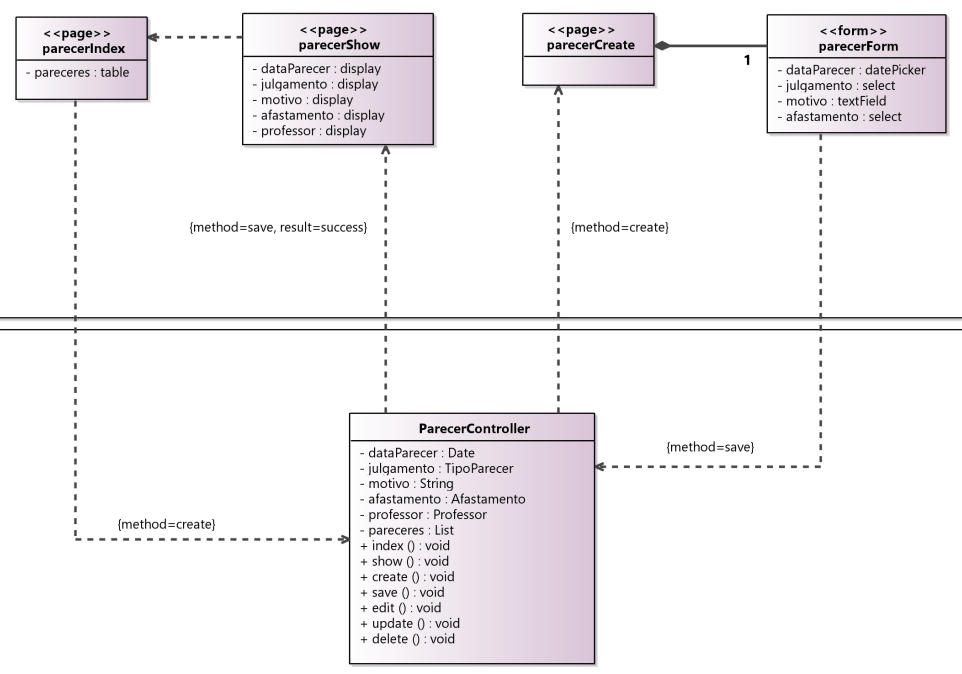
\includegraphics[width=1\textwidth]{figuras/fig-projeto-defParecer_manifContra.png}
	\caption{Modelo de Navegação dos Casos de Uso: Deferir Parecer e Manifestar-se Contra Afastamento.}
	\label{fig-projeto-defParecer_manifContra}
\end{figure}

Os casos de uso ``Cancelar Afastamento'', ``Arquivar Afastamento'', ``Registrar Parecer CT'' e ``Registrar Parecer PRPPG'' também são bem parecidos. Um professor cancela um pedido de afastamento realizando a alteração da situação da solicitação. Do mesmo modo, um secretário realiza a mudança da situação da solicitação, quando necessita arquivar um afastamento, registrar um parecer do CT ou registrar um parecer da PRPPG. Assim, esses casos de uso foram apresentados na Figura~\ref{fig-projeto-cancelar_arquivar_CT_PRPPG}.   

\begin{figure}[!h]
	\centering
	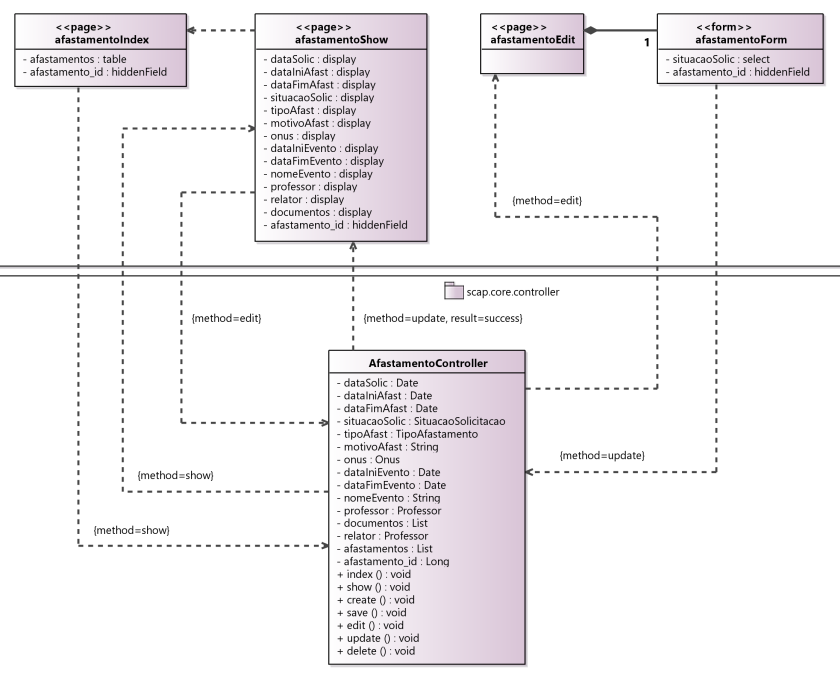
\includegraphics[width=1\textwidth]{figuras/fig-projeto-cancelar_arquivar_CT_PRPPG.png}
	\caption{Modelo de Navegação dos Casos de Uso: Cancelar Afastamento, Arquivar Afastamento, Registrar Parecer CT e Registrar Parecer PRPPG.}
	\label{fig-projeto-cancelar_arquivar_CT_PRPPG}
\end{figure}

Todos os usuários do sistema podem utilizar o caso de uso ``Consultar Afastamento''. Para isso, é possível filtrar a lista de afastamentos através de quatro buscas diferentes. O caso de uso está representado através da Figura~\ref{fig-projeto-consultarAfastamento}.

\begin{figure}[!h]
	\centering
	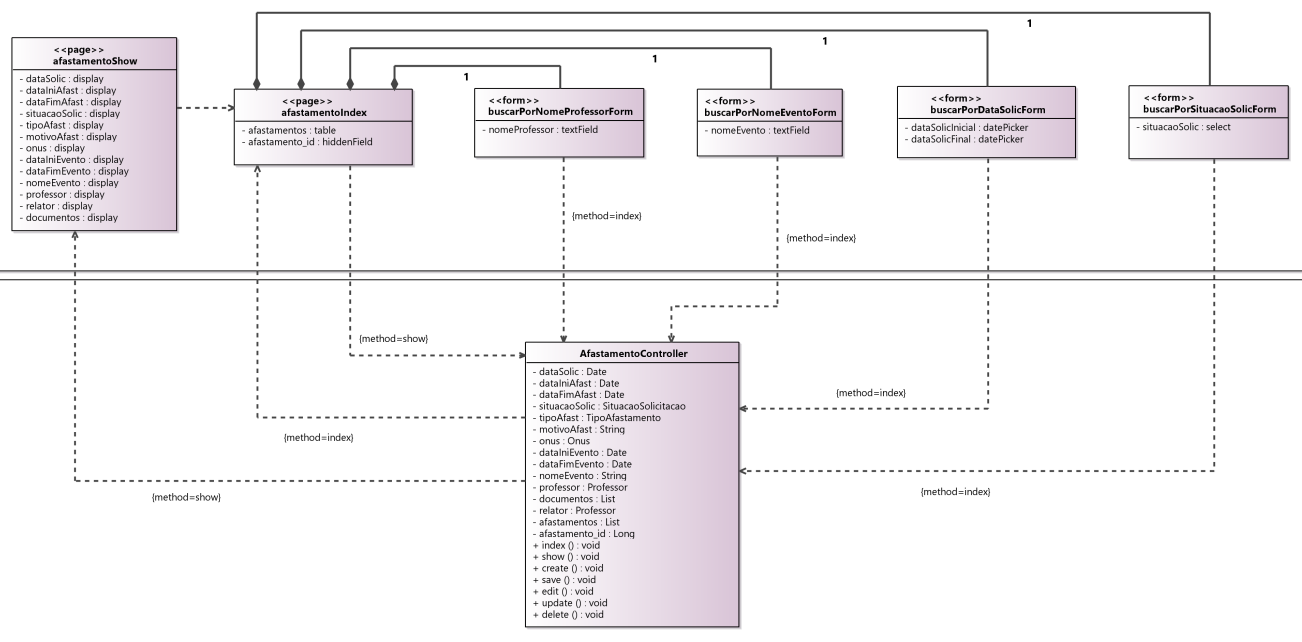
\includegraphics[width=1\textwidth]{figuras/fig-projeto-consultarAfastamento.png}
	\caption{Modelo de Navegação do Caso de Uso: Consultar Afastamento.}
	\label{fig-projeto-consultarAfastamento}
\end{figure}

% Impede os modelos de navegação de invadir a seção seguinte.
\FloatBarrier

\subsection{Modelo de Entidades}
\label{sec-projeto-modelo-entidades}

Utilizando o diagrama de classes que já foi apresentado na Figura~\ref{fig-requisitos-diagrama-classes}, o Modelo de Entidades recebeu uma adequação de acordo com a plataforma de implementação utilizada. Foram especificados os tipos de dados de cada atributo, assim como as definições das navegabilidades das associações, mapeamentos de persistência, entre outras coisas. Esta adequação pode ser visualizada através da Figura~\ref{fig-projeto-entidades}, que representa o Modelo de Entidades do SCAP.

No modelo é possível observar o tipo referente a cada atributo, se ele pode ser inicializado com o valor nulo ou não, assim como alguns mapeamentos objeto/relacionais, como por exemplo: o valor ``timestamp'' que indica que um atributo do tipo ``Date'' pode armazenar a data e a hora. Ainda é possível visualizar os tipo de dados enumerados do sistema, que estão representados na Figura~\ref{fig-projeto-enum}. Os tipos enumerados utilizados neste projeto foram os mesmo que estavam presentes na versão do SCAP que foi reformulada por~\citeonline{prado-pg15}, sendo necessário acrescentar o \textbf{TipoCargo}, que pode assumir os valores PROFESSOR ou SECRETARIO. Ambos os valores podem ser utilizados na classe pessoa que é persistida no banco de dados.   

\begin{figure}[!h]
	\centering
	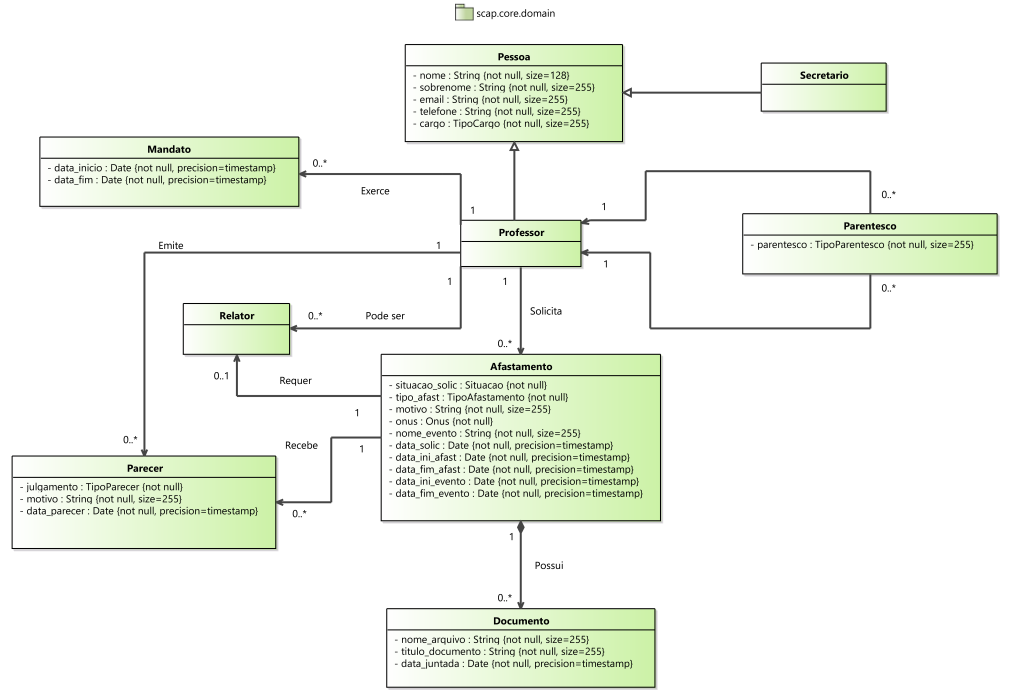
\includegraphics[scale=0.45]{figuras/fig-projeto-entidades} 
	\caption{Modelo de Entidades do SCAP.}
	\label{fig-projeto-entidades}
\end{figure}

\begin{figure}[!h]
	\centering
	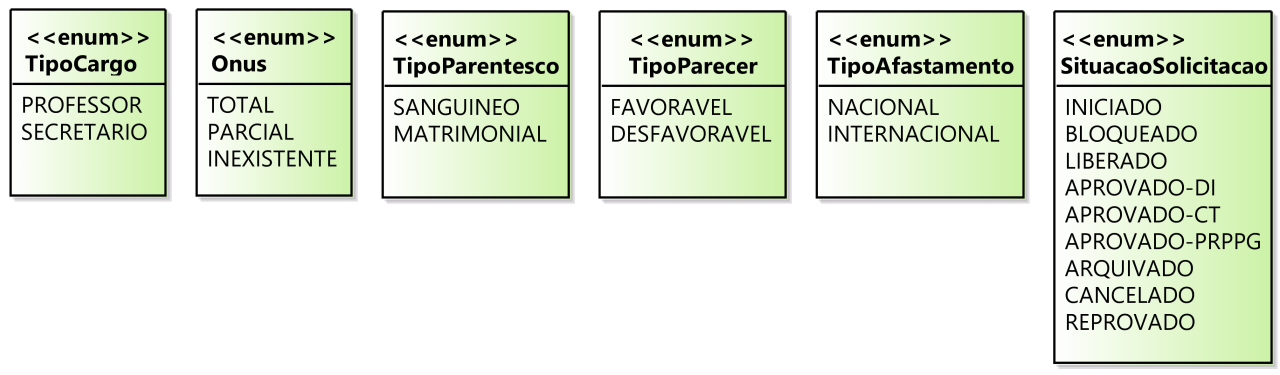
\includegraphics[scale=0.3]{figuras/fig-projeto-enum} 
	\caption{Tipos Enumerados do SCAP.}
	\label{fig-projeto-enum}
\end{figure}

\subsection{Modelo de Aplicação}
\label{sec-projeto-modelo-aplicacao}

Neste projeto foi gerado um modelo de aplicação que representa quais classes de ação que dependem de quais classes de serviço e quais \textit{Data Access Object} (DAO) foram utilizados. Portanto, este modelo pode ser visualizado através da Figura~\ref{fig-projeto-aplicacao1} e da Figura~\ref{fig-projeto-aplicacao2}. 

\begin{figure}[!h]
	\centering
	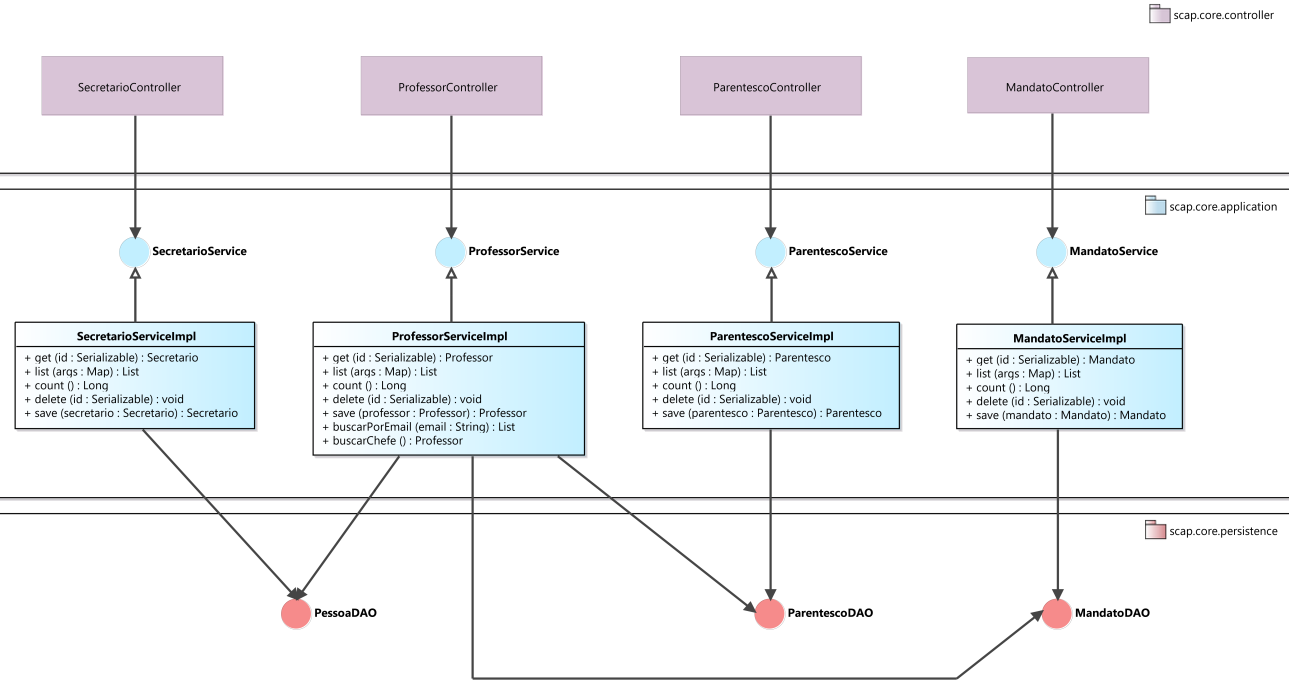
\includegraphics[width=1\textwidth]{figuras/fig-projeto-aplicacao1.png}
	\caption{Modelo de Aplicação - Parte 1.}
	\label{fig-projeto-aplicacao1}
\end{figure}

\begin{figure}[!h]
	\centering
	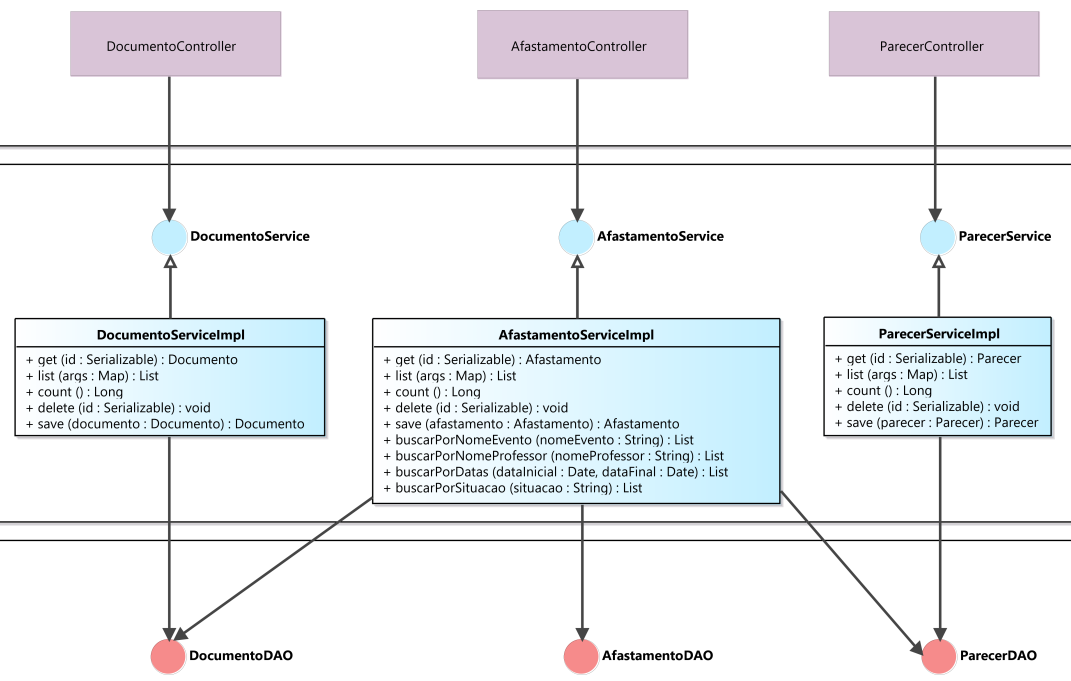
\includegraphics[width=1\textwidth]{figuras/fig-projeto-aplicacao2.png}
	\caption{Modelo de Aplicação - Parte 2.}
	\label{fig-projeto-aplicacao2}
\end{figure}
   

\subsection{Modelo de Persistência}
\label{sec-projeto-modelo-persistencia}

As classes DAO que fazem parte do pacote Persistência, são construídas com o auxílio deste diagrama que pode ser visualizado por meio da Figura~\ref{fig-projeto-persistencia}.
Para cada classe de domínio que precisa de lógica de acesso a dados, foi criada uma interface e uma classe concreta DAO que realiza a implementação dessa interface. A partir da criação da interface DAO base, todas as outras interfaces herdaram as definições e as implementações concretas que foram definidas.

De acordo com o método FrameWeb~\cite{souza:masterthesis07,souza-celebratingfalbo20}, é aconselhável seguir um padrão de nomes para as classes DAO, sendo que as intefaces devem seguir o padrão \textbf{<nome da classe de domínio>DAO} e as classes concretas devem seguir o padrão \textbf{<nome da interface><tecnologia de persistência>}. O \textit{framework} Grails que foi utilizado neste projeto utiliza o \textbf{GORM} como tecnologia de persistência. A tecnologia \textbf{GORM} já foi descrita anteriormente na subseção~\ref{sec-projeto-gorm}.

Para evitar a poluição visual no Modelo de Persistência, não existe uma representação explícita da relação de herança entre o DAO base e os DAOs específicos. Através da definição de padrões, o foco é estabelecer regras para que a modelagem se torne mais simples e mais rápida.    

\begin{figure}[!h]
	\centering
	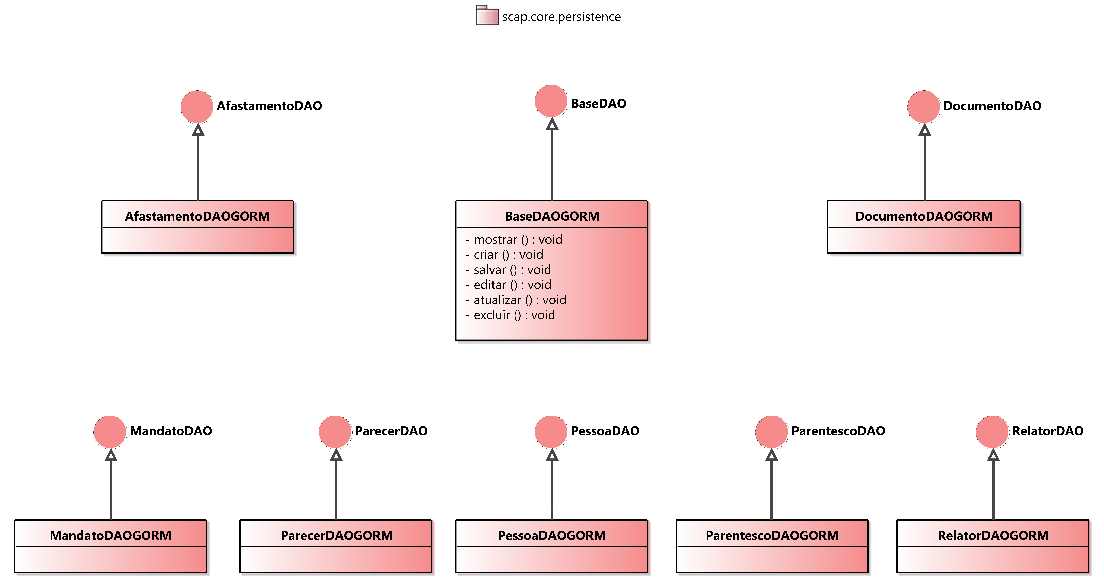
\includegraphics[scale=0.45]{figuras/fig-projeto-persistencia} 
	\caption{Modelo de Persistência do SCAP.}
	\label{fig-projeto-persistencia}
\end{figure}

\section{Exibição do Sistema}
\label{sec-projeto-exibicao-sistema}

O sistema possui um controle de segurança através da autenticação de usuários, não sendo possível acessar o conteúdo das páginas modificando a URL (\textit{Uniform Resource Locator}) do navegador utilizado. Para ter acesso ao sistema, o usuário deve fornecer o login e a senha que são cadastrados pelos administradores do sistema. Na Figura~\ref{fig-projeto-login} é possível visualizar a tela de login.   

\begin{figure}[!h]
	\centering
	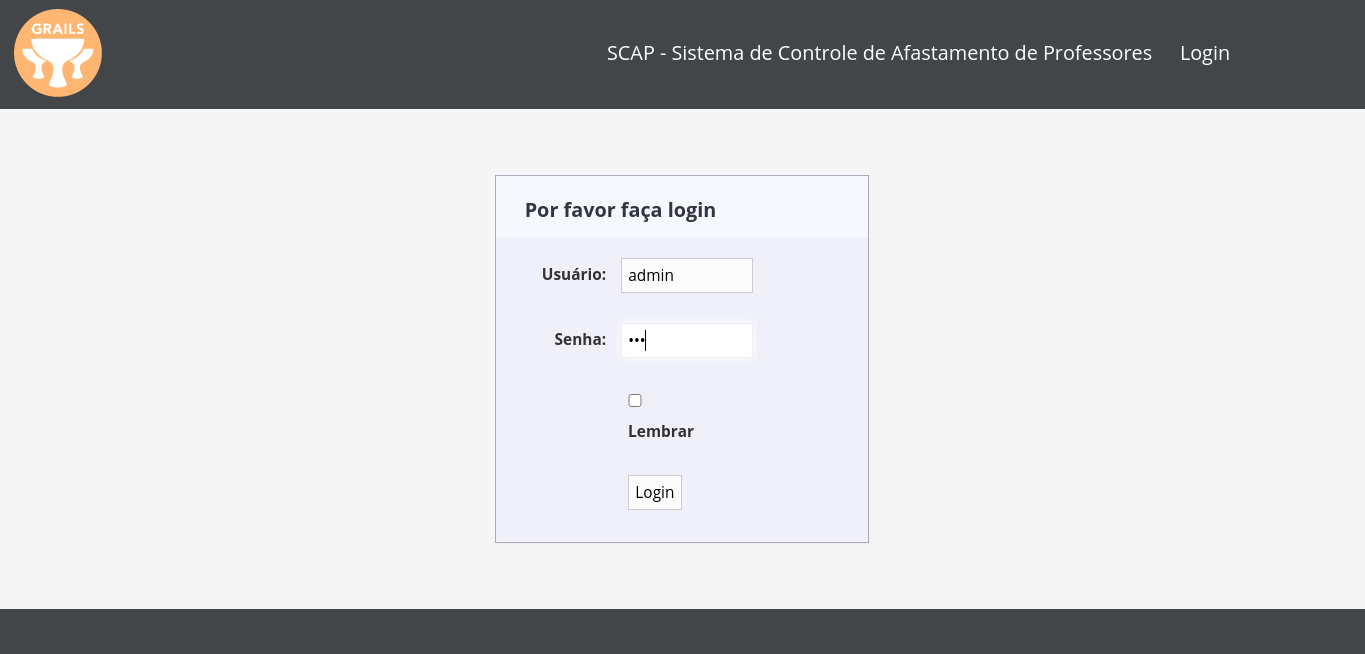
\includegraphics[scale=0.33]{figuras/fig-projeto-login} 
	\caption{Tela de Login do SCAP.}
	\label{fig-projeto-login}
\end{figure}

Por meio de regras de permissão, cada usuário visualiza a tela inicial de uma maneira modificada. Os secretários possuem a regra de permissão de administrador, pois são responsáveis pelo controle da maioria das funcionalidades. Já os professores possuem a regra de permissão de usuário, podendo visualizar as funcionalidades correspondentes ao seu cargo. O professor que se tornar chefe ou subchefe do departamento, pode visualizar todas as funcionalidades referentes aos professores e ainda pode cadastrar relatores para afastamentos internacionais. A Figura~\ref{fig-projeto-usuario-secretario} demonstra um usuário secretário que possui a regra de permissão de administrador. Na parte inferior da página do sistema, ficam localizados os botões chamados de controladores. Através deles é possível realizar as ações disponíveis por cada funcionalidade, como a realização de cadastramentos e as suas devidas associações. 

\begin{figure}[!h]
	\centering
	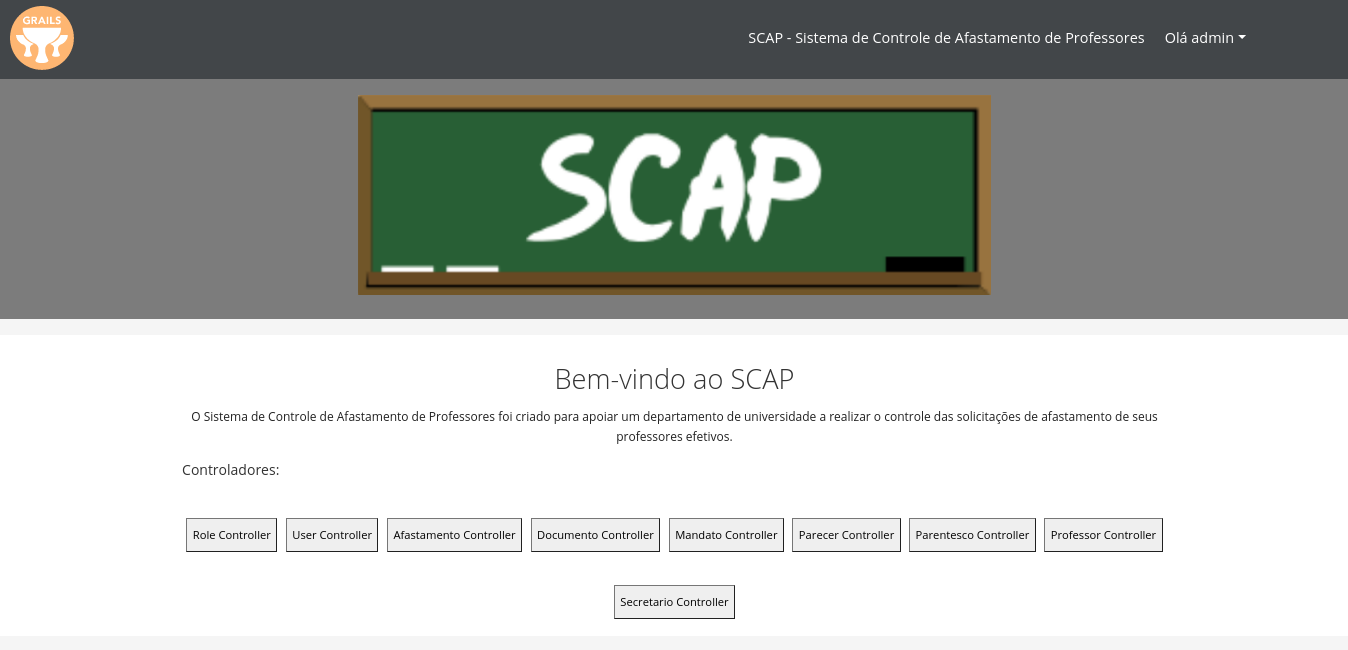
\includegraphics[scale=0.33]{figuras/fig-projeto-usuario-secretario} 
	\caption{Tela Inicial do Usuário Secretário do SCAP.}
	\label{fig-projeto-usuario-secretario}
\end{figure}

Ao clicar no botão ``Professor Controller'', o usuário secretário é redirecionado para a página de cadastramento de professores, pois cabe a ele cadastrar todos os professores e os parentescos entre eles. Para cadastrar os parentescos, o botão ``Parentesco Controller'' deve ser acionado, sendo necessário informar se o parentesco é sanguíneo ou matrimonial. As Figuras~\ref{fig-projeto-cadastrar-professor} e~\ref{fig-projeto-cadastrar-parentesco} demonstram essas funcionalidades.

\begin{figure}[!h]
	\centering
	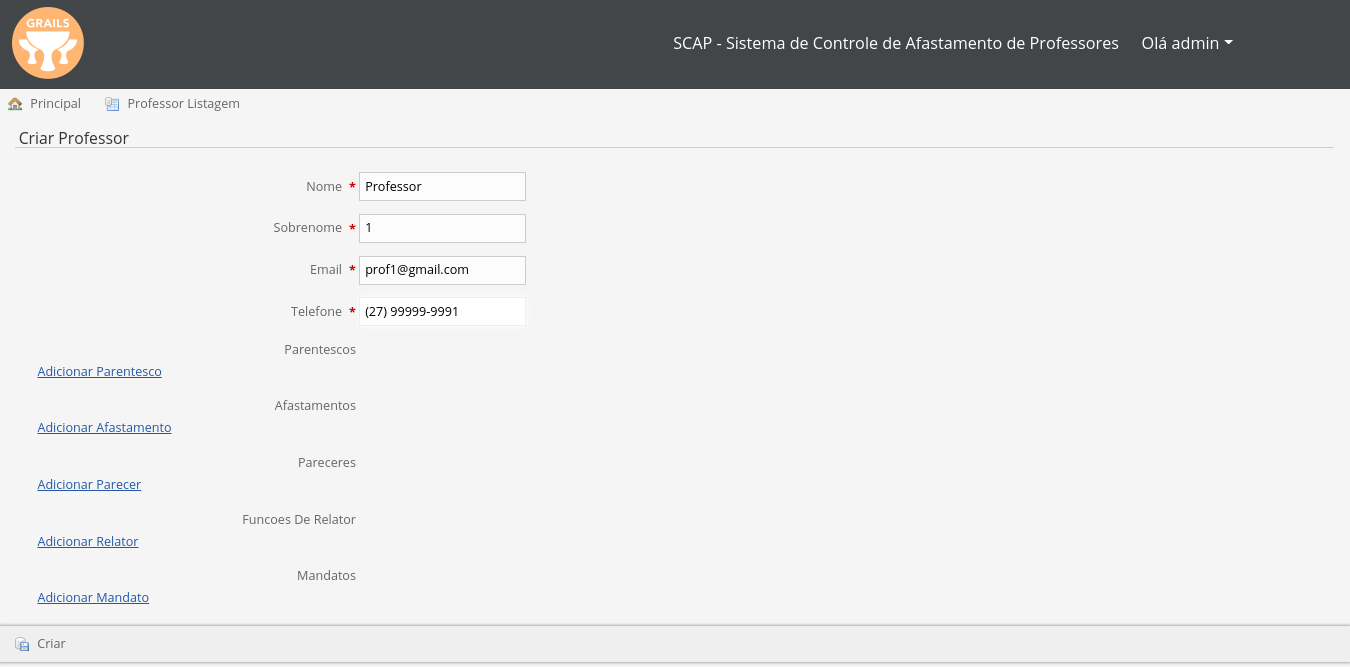
\includegraphics[scale=0.33]{figuras/fig-projeto-cadastrar-professor} 
	\caption{Tela Cadastrar Professor do SCAP.}
	\label{fig-projeto-cadastrar-professor}
\end{figure}

\begin{figure}[!h]
	\centering
	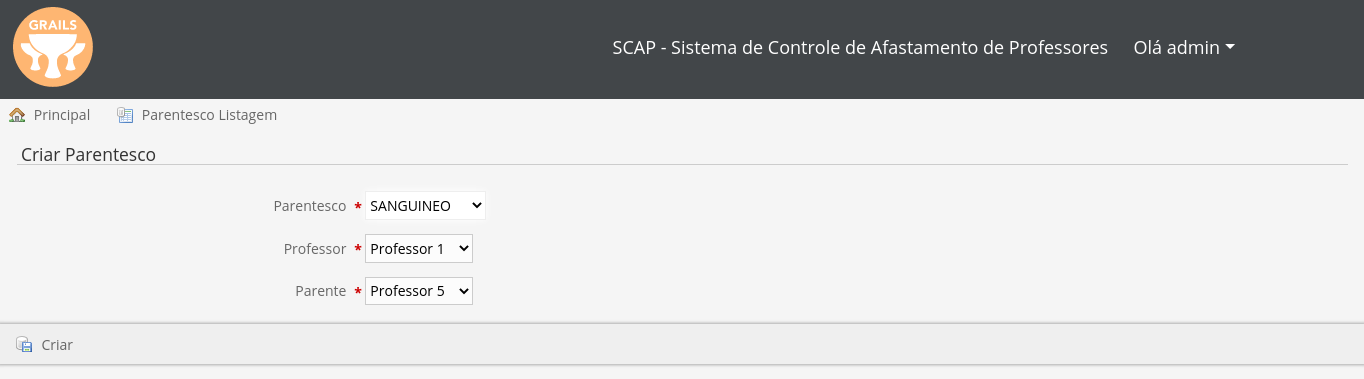
\includegraphics[scale=0.33]{figuras/fig-projeto-cadastrar-parentesco} 
	\caption{Tela Cadastrar Parentesco do SCAP.}
	\label{fig-projeto-cadastrar-parentesco}
\end{figure}

O usuário secretário também tem a responsabilidade de realizar o cadastramento do mandato referente ao chefe ou subchefe do departamento. Para aplicar esta ação, é necessário utilizar o botão ``Mandato Controller'', onde o secretário será redirecionado para a página de cadastro, sendo possível informar o período referente ao mandato e também selecionar o professor na lista de professores cadastrados. Este cadastramento pode ser visualizado através da Figura~\ref{fig-projeto-cadastrar-mandato}. 

\begin{figure}[!h]
	\centering
	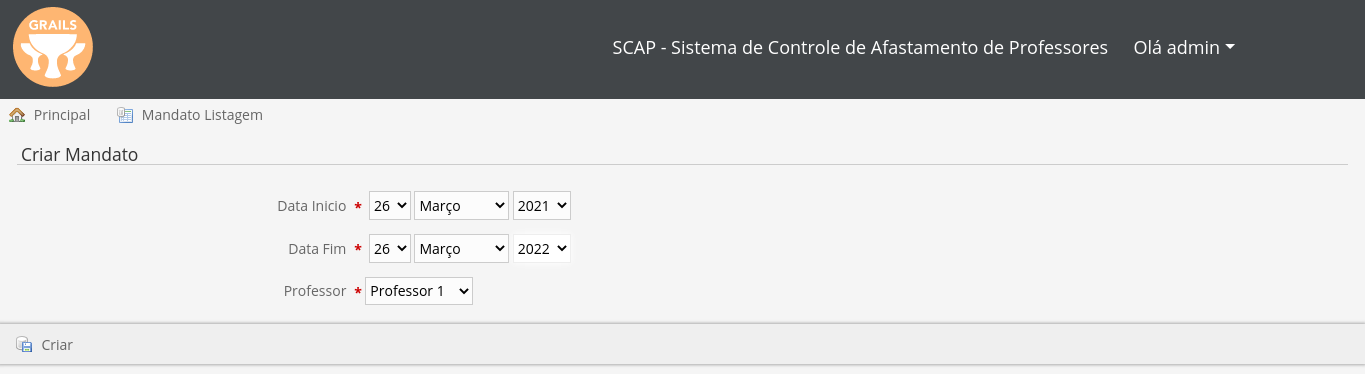
\includegraphics[scale=0.33]{figuras/fig-projeto-cadastrar-mandato} 
	\caption{Tela Cadastrar Mandato do Chefe de Departamento do SCAP.}
	\label{fig-projeto-cadastrar-mandato}
\end{figure}

Após o secretário realizar o cadastramento dos professores, o cadastramento dos parentescos e o cadastramento do mandato referente ao chefe ou subchefe do departamento, os professores recebem o acesso ao sistema. Por possuírem a regra de permissão de usuário, os professores visualizam a tela inicial com as funcionalidades reduzidas. A tela inicial do usuário professor pode ser visualizada através da Figura~\ref{fig-projeto-usuario-professor}. 

\begin{figure}[!h]
	\centering
	
\includegraphics[scale=0.33]{figuras/fig-projeto-usuario-professor} 
	\caption{Tela Inicial do Usuário Professor do SCAP.}
	\label{fig-projeto-usuario-professor}
\end{figure}

A Figura~\ref{fig-projeto-cadastrar-afastamento} demonstra a principal funcionalidade do sistema. Ao clicar no botão ``Afastamento Controller'' o professor pode preencher todas as informações necessárias para realizar uma solicitação de afastamento, iniciando todo o processo para que as tramitações sejam aplicadas. Através do botão ``Documento Controller'', é possível cadastrar documentos para que eles sejam associados ao afastamento. Está funcionalidade é demonstrada por meio da Figura~\ref{fig-projeto-cadastrar-documento}.   

\begin{figure}[!h]
	\centering
	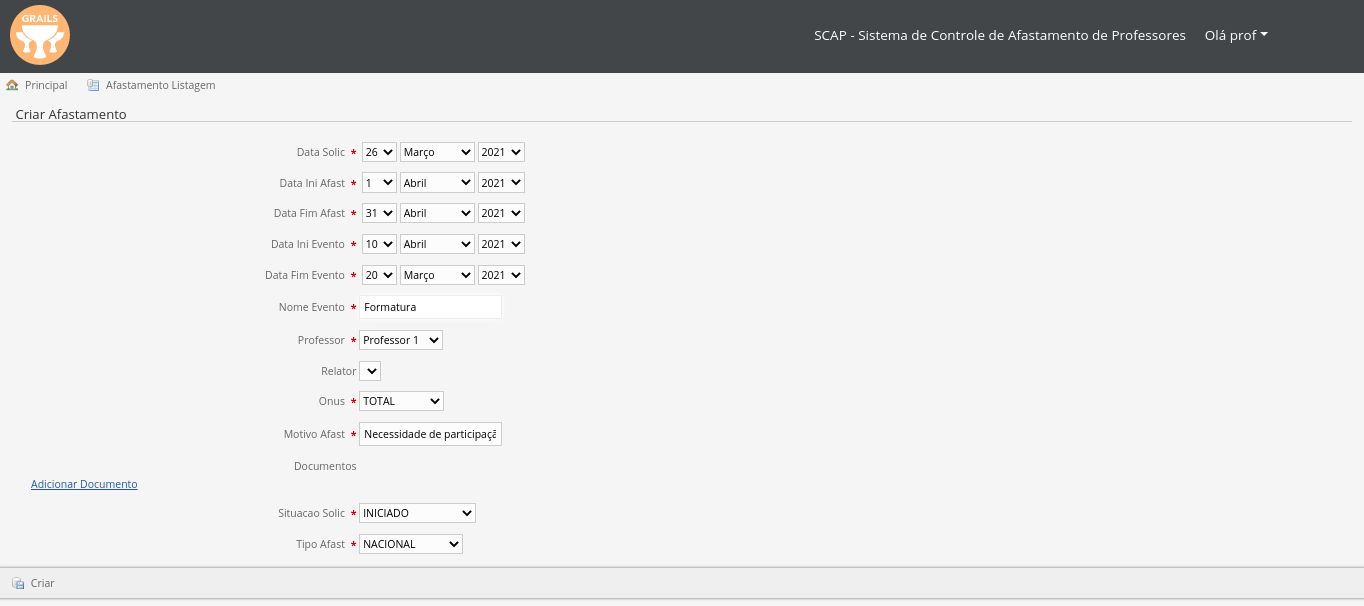
\includegraphics[scale=0.33]{figuras/fig-projeto-cadastrar-afastamento} 
	\caption{Tela Cadastrar Afastamento do SCAP.}
	\label{fig-projeto-cadastrar-afastamento}
\end{figure}

\begin{figure}[!h]
	\centering
	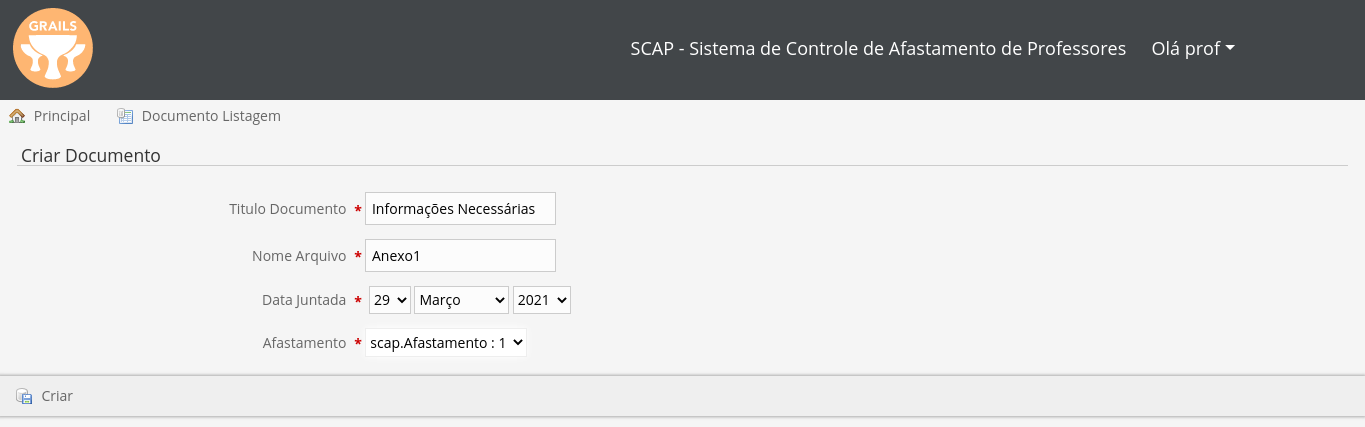
\includegraphics[scale=0.33]{figuras/fig-projeto-cadastrar-documento} 
	\caption{Tela Cadastrar Documento de um Afastamento do SCAP.}
	\label{fig-projeto-cadastrar-documento}
\end{figure}

O cadastro de um parecer é exemplificado pela Figura~\ref{fig-projeto-cadastrar-parecer}. Utilizando o botão ``Parecer Controller'', o professor que foi cadastrado pelo chefe do departamento como sendo relator de uma solicitação de afastamento internacional, pode preencher as informações justificando o motivo da sua decisão. Caso um professor seja contra a alguma solicitação de afastamento, ele também pode cadastrar um parecer. 

\begin{figure}[!h]
	\centering
	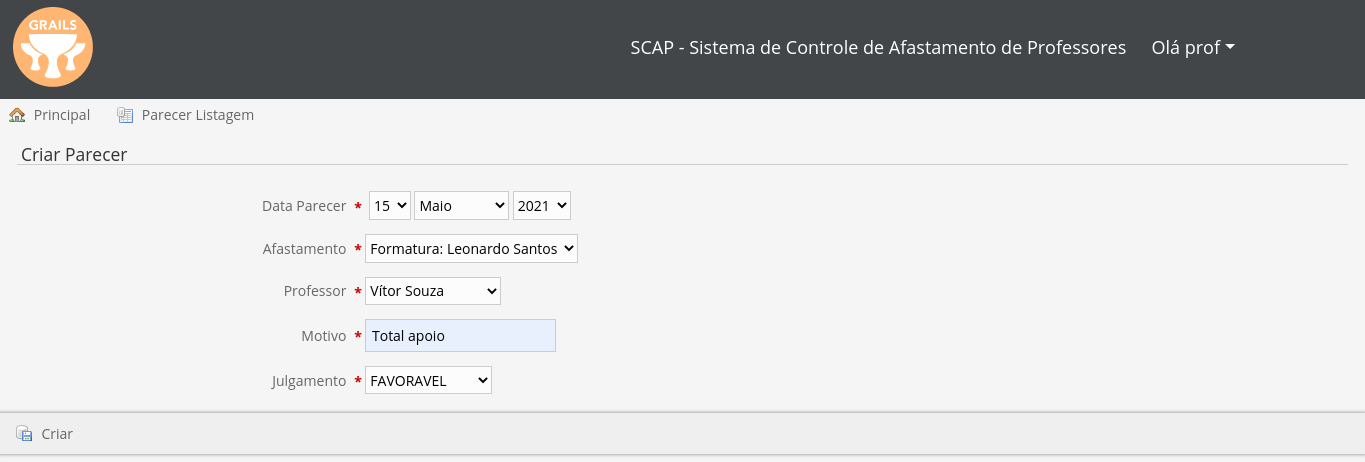
\includegraphics[scale=0.33]{figuras/fig-projeto-cadastrar-parecer} 
	\caption{Tela Cadastrar Parecer de um Afastamento do SCAP.}
	\label{fig-projeto-cadastrar-parecer}
\end{figure}

Todos os usuários do sistema podem realizar consultas para obterem informações sobre uma solicitação de afastamento. Os usuários podem realizar buscas pelo nome do professor, pelo nome do evento, pela situação do afastamento ou pelo período de data de solicitação. É possível visualizar uma lista com todos os afastamentos cadastrados no sistema e também obter detalhes de um afastamento específico. A Figura~\ref{fig-projeto-listar-afastamentos} apresenta a lista contendo todos os afastamentos e a Figura~\ref{fig-projeto-ver-afastamento} exibe os detalhes do afastamento selecionado.  

\begin{figure}[!h]
	\centering
	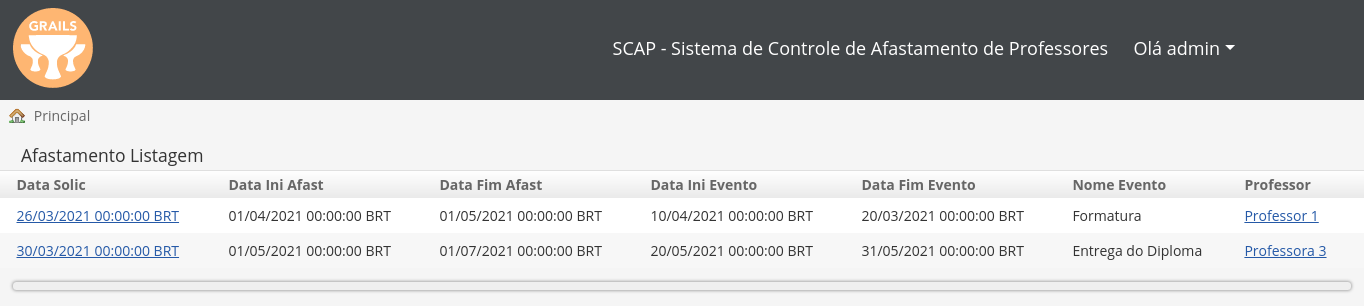
\includegraphics[scale=0.33]{figuras/fig-projeto-listar-afastamentos} 
	\caption{Tela Listar Afastamentos do SCAP.}
	\label{fig-projeto-listar-afastamentos}
\end{figure}

\begin{figure}[!h]
	\centering
	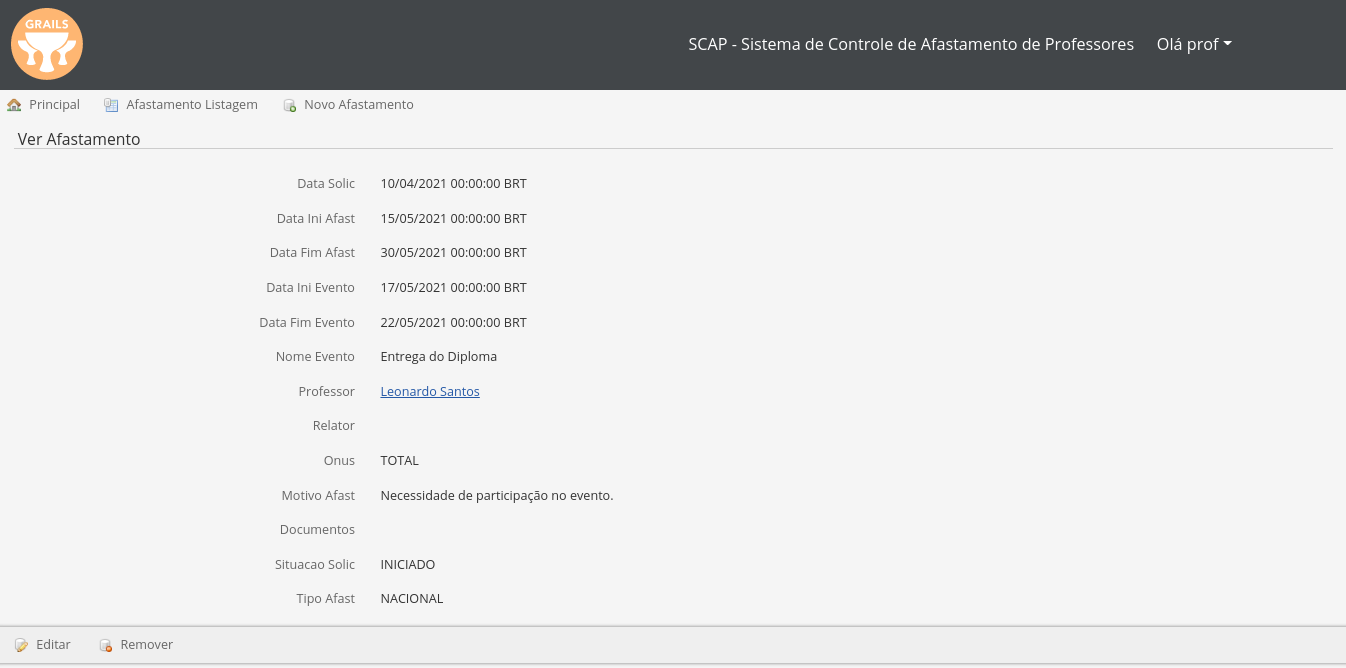
\includegraphics[scale=0.33]{figuras/fig-projeto-ver-afastamento} 
	\caption{Tela Visualizar Afastamento do SCAP.}
	\label{fig-projeto-ver-afastamento}
\end{figure}

A Figura~\ref{fig-projeto-listar-professores} demonstra mais uma funcionalidade disponível para o usuário secretário. Para melhorar o controle, é possível visualizar uma lista contendo todos os professores cadastrados, assim como os seus respectivos parentescos. Além disso, é possível saber de todas as solicitações de afastamentos realizadas por cada professor e realizar uma busca por email.  

\begin{figure}[!h]
	\centering
	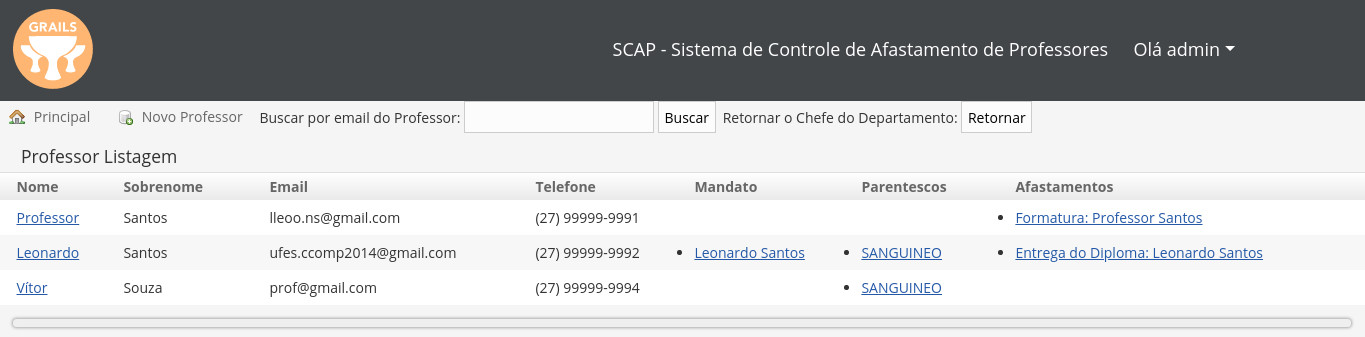
\includegraphics[scale=0.33]{figuras/fig-projeto-listar-professores} 
	\caption{Tela Listar Professores do SCAP.}
	\label{fig-projeto-listar-professores}
\end{figure}

Após as tramitações de um afastamento serem realizada, o usuário secretário deve efetuar uma atualização no afastamento cadastrado, fazendo uma modificação no status do mesmo. Para isso, ele deve editar o afastamento, mudando o campo ``Situacao Solic'' para ``Arquivado''. Por fim, a Figura~\ref{fig-projeto-editar-afastamento} exemplifica esta ação.

\begin{figure}[!h]
	\centering
	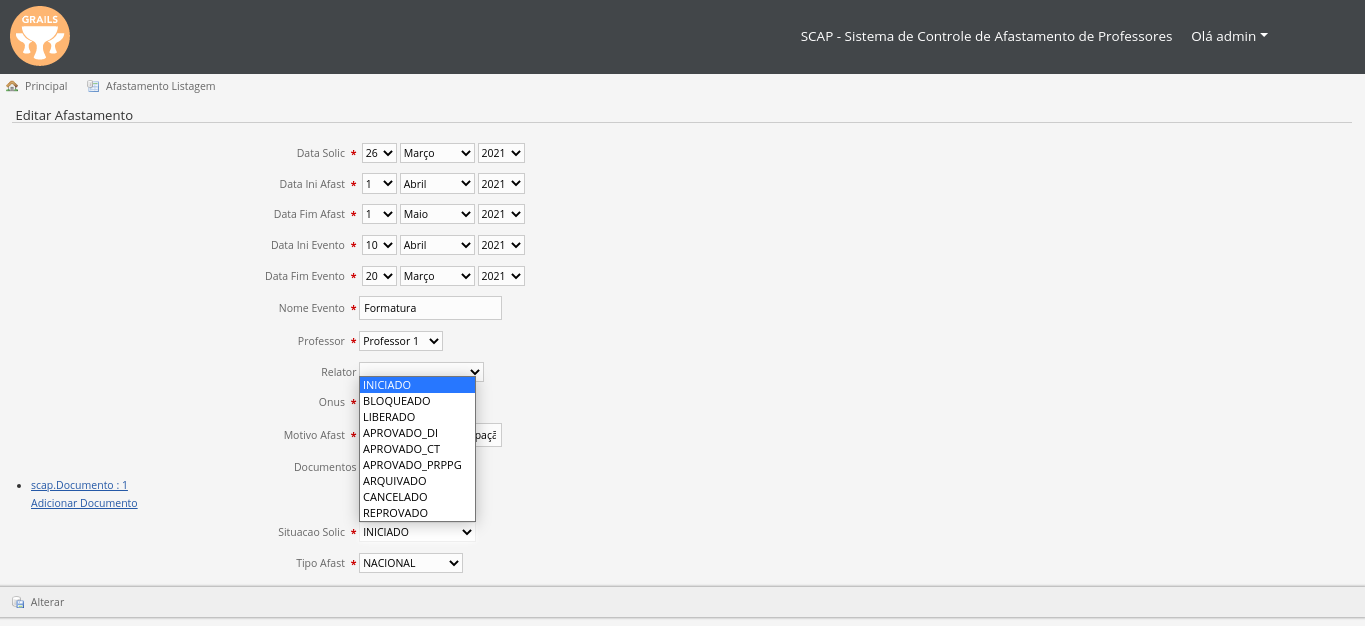
\includegraphics[scale=0.33]{figuras/fig-projeto-editar-afastamento} 
	\caption{Tela Editar Afastamento do SCAP.}
	\label{fig-projeto-editar-afastamento}
\end{figure}

% ==============================================================================
% TCC - Nome do Aluno
% Capítulo 5 - Considerações Finais
% ==============================================================================
\chapter{Considerações Finais}
\label{sec-conclusoes}

Para que os objetivos fossem alcançados, foi preciso combinar todo o conhecimento adquirido durante o curso, reunindo o aprendizado obtido nas disciplinas de Banco de Dados, Linguagens de Programação, Engenharia de \textit{Software}, Desenvolvimento \textit{Web} e \textit{Web} Semântica, entre outras. Através deste conhecimento, foi possível estabelecer a melhor estratégia para que os problemas enfrentados durante o projeto fossem sanados, gerando soluções que se tornaram bastante satisfatórias.  

A versão do sistema SCAP descrita no decorrer deste projeto foi implementada utilizando a linguagem Apache Groovy que ainda não tinha sido utilizada em versões anteriores. Por este motivo, é importante ressaltar que não foi utilizado nenhum código que estava presente nas versões passadas. Assim, foi necessário realizar o estudo e aprendizagem da linguagem Groovy e do \textit{framework} Grails para que eles pudessem ser utilizados. O aprendizado de uma nova linguagem é um desafio que proporciona um retorno muito grande, agregando muita experiência que pode ser aplicada em diversas áreas.

Com a utilização de um \textit{framework}, a implementação do sistema SCAP se tornou uma tarefa bem mais simples do que se fosse necessário implementar todo o código sem ter uma base de início. Além de fornecer a geração de boa parte do código necessário para o funcionamento do sistema, o \textit{framework} ainda disponibiliza diversas bibliotecas que podem ser incluídas no projeto a qualquer momento, diminuindo o tempo e as complexidades do desenvolvimento.  

Durante o aprendizado para a utilização do \textit{framework} Grails, algumas dificuldades foram enfrentadas. Apesar do \textit{framework} disponibilizar uma rica documentação, alguns fatores são explicados de forma superficial, como por exemplo, a conexão com um banco de dados relacional. Para essa tarefa foi necessário recorrer aos fóruns da comunidade do \textit{framework}, assim como vídeos tutoriais encontrados na \textit{internet}. Outra dificuldade enfrentada foi a incompatibilidade entre as versões do \textit{framework}. Basta atualizar a versão e o projeto deixa de funcionar, sendo necessário realizar muitas alterações para que os erros sejam solucionados.

Depois que~\citeonline{souza:masterthesis07} estabeleceu uma organização para os \textit{frameworks} em categorias diferentes, realizar a escolha de um \textit{framework} que se enquadre na execução das propostas de um projeto se tornou uma tarefa bem mais fácil. Com a aplicação do método FrameWeb na fase de projeto arquitetural, a criação de modelos de projeto se aproxima muito da implementação do sistema, definindo uma arquitetura básica e deixando os desenvolvedores livres para adotarem as técnicas mais adequadas para as outras etapas do processo.

Para a criação dos modelos que são propostos pelo método FrameWeb, foi utilizada a ferramenta FrameWeb \textit{Editor}~\cite{campos-souza:webmedia17}. Nesta etapa, foi necessário realizar a instalação e configuração da ferramenta, seguindo o tutorial~\cite{souza:ftt21} referente a ela. As configurações são um pouco extensas e devem ser realizadas com bastante atenção para evitar possíveis erros. No tutorial também são listadas algumas dicas para resolver erros que podem aparecer durante as configurações.

A utilização do FrameWeb \textit{Editor} não é muito intuitivo no início, mas com relação as funcionalidades, a ferramenta cumpre o seu propósito. É possível realizar a criação dos quatro tipos básicos de modelos FrameWeb, fazendo verificações nos modelos e impedindo ações inválidas. Como toda ferramenta criada recentemente, ainda é necessário realizar correções em alguns erros, como por exemplo, o salvamento das associações entre os elementos contidos no modelo de navegação. Com o lançamento de novas versões da ferramenta, certamente esses erros serão solucionados.

Realizando a aplicação do método FrameWeb, claramente a sua eficiência e eficácia ficaram comprovadas. Por meio dos modelos que foram gerados, a implementação do código do sistema através do \textit{framework} Grails foi agilizada, sendo necessário apenas seguir com as etapas do projeto. Com a divisão do sistema em camadas, a organização e a modularização tornaram os componentes do SCAP bem mais fáceis de serem aperfeiçoados ou substituídos.                          

\section{Trabalhos Futuros}
\label{sec-conclusoes-trabalhos-futuros}

Texto



%%% Páginas finais do documento: bibliografia e anexos. %%%

% Finaliza a parte no bookmark do PDF para que se inicie o bookmark na raiz e adiciona espaço de parte no sumário.
\phantompart

% Marca o início dos elementos pós-textuais.
\postextual

% Referências bibliográficas
\bibliography{bibliografia}


% Apêndices.
\begin{apendicesenv}

% Imprime uma página indicando o início dos apêndices.
\partapendices

% (*) Incluir como apêndice a documentação técnica produzida durante o PG (especificação de requisitos,
% projeto arquitetural, etc.). Utilizar o exemplo \includepdf caso o documento seja produzido em outro
% editor de texto (Microsoft Word, LibreOffice Writer) e transformado em PDF. Utilizar o exemplo \include
% caso os documentos tenham sido também escritos em LaTeX.
% \includepdf[pages={1-}]{apendices/apendice01-requisitos.pdf}
% \includepdf[pages={1-}]{apendices/apendice02-projeto.pdf}
% \include{ap1-requisitos}
% \include{ap2-projeto}
\end{apendicesenv}


% Índice remissivo.
\phantompart
\printindex

% Fim do documento.
\end{document}
